%----------------------------------------------------------------------------------------------------
%							Preamble
%----------------------------------------------------------------------------------------------------


\documentclass[fontsize=12pt,headsepline=true, bibliography=totocnumbered, twoside]{scrbook} % remove 'bibliography=totocnumbered' to not show bibliography in table of contents. 'headsepline=true' creates line under headers. 'twoside' option sets for new chapters to begin on right side of the book; to not have empty pages change it to 'oneside'. 'fontsize=12pt' sets font size. check documentation for available option for scrbook class


\addtokomafont{disposition}{\rmfamily} % to change font to roman font



\usepackage[a4paper, bottom=40mm, bindingoffset=6mm]{geometry} % defines geometry of the thesis

\usepackage{setspace} % used to set line spacing
\linespread{1.25} % change value to have different line spacing

\usepackage{booktabs} % used to create tables

\usepackage[colorlinks=true, allcolors=black]{hyperref} % used for cross referencing. 'colorlinks=true' will color the references. for custom color options check documentation

\usepackage[dvipsnames,table,xcdraw]{xcolor} %used to colour text and tables. Look up documentation for available options


\usepackage{graphicx} % used to insert pictures. jpg, png, pdf and eps format is supported. check documentation for more details

\graphicspath{{images/}} % path of images

\usepackage{caption} % used for captions for figures and tables
\usepackage{subcaption} % used for subcaptions for figures and tables


\usepackage[square,numbers,sort&compress]{natbib} % used for bibliography. 'square' options puts square brackets on citations. can be changed to 'round' for round brackets. 'super' option can be used for having citations as superscript. 'numbers' option numbers it. check documentation for more options





\usepackage[printonlyused,withpage]{acronym} % used for creating acronyms/abbreviations. 'withpage' option gives page number



\usepackage[T1]{fontenc}
\usepackage[main=english,polish]{babel}
\usepackage[utf8]{inputenc}
\usepackage{lmodern}

\usepackage{microtype} % to improve hypenation




%--------------------------------------------------------------------------------------------------


\begin{document}



%----------------------------------------------------------------------------------------------------
%						Title page in polish
%----------------------------------------------------------------------------------------------------



\begin{titlepage}

\newgeometry{centering,margin=2cm, bindingoffset=6mm} % correct binding offset if necessary
    \begin{center}     
        \vspace*{1cm}
        \Huge 
        \textbf{UNIWERSYTET ~WROC\L{}AWSKI}
        
        
        \LARGE 
        \textbf{Wydział Biotechnologii}

		\Large 
		\textbf{Medical Biotechnology}
            
        \vspace{3.5cm}
            
       {\color {Blue}{\LARGE {\textbf{Rakshith Suhas Charles}}}} % Add your name here
       
       \vspace{1.5cm}
       
       {\color {Blue}{\LARGE{Identyfikacja archeonów potencjalnie zdolnych do bezpośredniego wychwytu elektronów}}} % Thesis title in polish here 
            
        \vspace{4cm}

{\Large  Praca magisterska wykonana w Zakładzie/Laboratorium: }



{\color {Blue}{\Large \bfseries Zakład Biotransformacji}} % name of the department in polish

\Large Opiekun pracy:{\color {Blue} \Large \bfseries ~ Dr Sławomir Jabłoński} % name of your guide
   
\vspace{3.5cm}

\LARGE \bfseries Wrocław, 2021-09-28   % Add date here       
       
           
\end{center}            
    
\end{titlepage}






%----------------------------------------------------------------------------------------------------
%						Title page in English
%---------------------------------------------------------------------------------------------------- 
 

\begin{titlepage}
\newgeometry{centering,margin=2cm, bindingoffset=6mm} % correct binding offset if necessary
    \begin{center}
         \vspace*{1cm}   
        \Huge
        \textbf{UNIVERSITY OF WROCLAW}     
        
        
        \LARGE
        \textbf{Faculty of Biotechnology}

		\Large
		\textbf{Medical Biotechnology}
            
        \vspace{3.5cm}
            
       {\color {Blue}{\LARGE {\textbf{Rakshith Suhas Charles}}}} % Add your name here
       
       \vspace{1.5cm}
       
       {\color {Blue}{\LARGE{ Identification of archaea potentially capable of direct electron uptake}}} % Thesis title in English
            
        \vspace{4cm}

{\Large  Master's thesis completed in the Department/Laboratory:}



{\color {Blue}{\Large \bfseries Department of Biotransformation}} % name of your department

\Large Supervisor:{\color {Blue} \Large \bfseries  ~ Dr. Sławomir Jabłoński} % name of your guide
   
\vspace{3.5cm}

\LARGE \bfseries Wroclaw, 2021-09-28   % Add date here             
       
           
\end{center}            
    
\end{titlepage} 
 


%----------------------------------------------------------------------------------------------------
%							Front Matter
%----------------------------------------------------------------------------------------------------






\frontmatter   % creates page number in roman numerals till main matter







%----------------------------------------------------------------------------------------------------
%						Abstract in Polish
%----------------------------------------------------------------------------------------------------





\chapter*{Streszczenie} %remove asterisk to show in table of contents

Fermentacja metanowa jest procesem biologicznym wykorzystywanym w stabilizacji odpadów bogatych w związki organiczne, przy  jednoczesnym wytwarzaniem biogazu. Szybkość tego procesu jest często ograniczona przez niskie tempo reakcji metabolicznych u mikroorganizmów syntroficznych. Stabilny i szybki transfer elektronów miedzy bakteriami octanogennymi i archeonami metanogennymi ma kluczowe znaczenie dla wydajnej metanogenezy. Przypuszczalnie  bezpośredni międzygatunkowy transfer elektronów jest metabolicznie bardziej korzystny w porównaniu z transferem pośrednim (opartym an wodorze lub kwasie mrówkowym). Jak do tej pory niewiele wiadomo na temat zdolności metanogenów do bezpośredniego międzygatunkowego transferu elektronów. Odkrycie elektrycznie przewodzącej archaelli u \textit{Methanospirillum hungatei} zasugerowało możliwość, że struktura ta może służyć do bezpośredniego wychwytu elektronów.\\ 
W ramach niniejszej pracy podjęto próbę identyfikacji archeonów metanogennych potencjalnie zdolnych do bezpośredniego wychwytu elektronów. Identyfikacja takich gatunków może pozwolić na uzyskanie populacji mikroorganizmów o wyższym potencjale metanogennym.
Przeprowadzone analizy wykazały obecność homologów białka tworzącego archaelli u archeonów metanogennych należących do klasy Methanomicrobia, w szczególności do rodzaju \textit{Methanosarcina}. Analiza danych literaturowych poddaje jednak w wątpliwość udział archaelli w procesie bezpośredniego wychwytu elektronów. Hipoteza alternatywna mówi, że za bezpośredni wychwyt elektronów są odpowiedzialne struktury powierzchniowe charakterystyczne dla mikroorganizmów z rzędu Methanosarcinales.






%----------------------------------------------------------------------------------------------------
%						Abstract in English
%----------------------------------------------------------------------------------------------------




\chapter*{Abstract} %remove asterisk to show in table of contents


Anaerobic digestion is an effective biological treatment for stabilizing organic compounds in wastes and in simultaneously producing biogas. It is often limited by the slow reaction rates of different microorganisms’ syntrophic biological metabolisms. Stable and fast interspecies electron transfer between acetogenic bacteria and methanogens is crucial for efficient methanogenesis. In particular, direct interspecies electron transfer has been proposed to be metabolically advantageous compared to mediated interspecies electron transfer via hydrogen or formate, but little is known about the diversity of methanogens capable of direct interspecies electron transfer. Discovery of electrically conductive archaella of \textit{Methanospirillum hungatei} suggested a possibility of archaella being a conduit for direct electron uptake. This study tried to explore this possibility and if true, as a conquence would lead to discovery of more methanogenic archae potentially capable of direct electron uptake.  In presented study archaella protein analogues were indentified in methanogenic archaea from Methanomicrobia class particularly \textit{Methanosarcina} genus. However analysis of available literature suggests that electrically conductive archaella may not play a direct role in electron uptake. Alternative hypothesis stands that direct electron uptake might be property of cell surface structures unique to methanogens of order Methanosarcinales.



%----------------------------------------------------------------------------------------------------
%				List of figures, tables and table of contents
%----------------------------------------------------------------------------------------------------




\tableofcontents % creates table of contents

\listoffigures   % creates list of figures

\listoftables    % creates list of tables


%----------------------------------------------------------------------------------------------------
%								List of Abbreviations
%----------------------------------------------------------------------------------------------------




\chapter*{List of Abbreviations} % Define list of abbreviations to be used later
	
\begin{acronym}[AAAAAAAA]\itemsep=1pt % [AAAAA] is to set indent. Only number of alphabet matters. \itemsep is to set line spacing
 		
 		\acro{AD}{Anaerobic digestion}
 		\acro{LCFAs}{Long chain fatty acids} 
 		\acro{VFAs}{Volatile fatty acids}
 		\acro{IET}{Interspecies electron transfer}
 		\acro{MIET}{Mediated interspecies electron transfer}
 		\acro{DIET}{Direct interspecies electron transfer}
 		\acro{AQDS}{Anthraquinone-2,6-disulfonate}
 		\acro{e-pili}{Electrically conductive pili}
 		\acro{CM}{Conductive material}
\acro{GAC}{Granular activated carbon}
\acro{OmcS}{Pilin associated c-type cytochrome} 

\acro{BRONJ}{Bisphosphonate-Related Osteonecrosis of the Jaw}
\acro{BLAST}{Basic local alignment search tool}
\acro{NCBI}{The National Center for Biotechnology Information}
\acro{MSA}{Multiple sequence alignment}
\acro{EMBL-EBI}{European Molecular Biology Laboratory-European Bioinformatics Institute}		
 
 		 	\end{acronym}
	
 		
 		
 		 	




%----------------------------------------------------------------------------------------------------
%								Main Matter
%----------------------------------------------------------------------------------------------------




\mainmatter % from here on arabic numerals will be used















\chapter{Introduction}


\section{Anaerobic digestion}

%1. Anaerobic digestion (microorganisms involved, interaction model between them).

\ac{AD} is the breakdown of organic material by microorganisms in the absence of oxygen. Although this takes place naturally in soils, sediments, ruminants, and several other anoxic environments, the term normally describes an artificially accelerated operation in closed vessels called anaerobic digesters, resulting in a relatively stable solid residue. Biogas is generated during \ac{AD} - mostly methane and carbon dioxide. This gas can be used as a chemical feedstock or as a fuel. \ac{AD} can treat many biodegradable wastes, including wastes that are unsuitable for composting, such as meat and cooked food\citep{nayono}.



\subsection{Historical perspective}

Anecdotal evidence indicates that biogas was used for heating bath water in Assyria during the
$10^{th}$ century BC and in Persia during the $16^{th}$ century. Methane generated during anaerobic processes was recorded as mysterious flickering flames in swamps and marshlands known as ``will-o-wisp''. Jean Baptiste Van Helmont in 1630 first determined that flammable gases could evolve from decaying organic matter. In 1776, Alessandro Volta concluded that there was a direct correlation between the amount of decaying organic matter and the amount of flammable gas emitted. He also determined that certain proportions of this flammable gas were explosive in air. In 1808, Humphry Davy determined that methane was present in the gases produced during the \ac{AD} of cattle manure. The first digestion plant was built at a leper colony in Bombay, India in 1859. In 1868, Bechamp, a student of Pasteur', attempted to isolate the microorganism responsible for the anaerobic bioconversion of ethanol to methane. In reality, Bechamp's attempts resulted in a co-culture of microorganisms.

The first practical application of \ac{AD} for energy production took place in England in 1896 when biogas from sewage sludge digestion was used to fuel street lamps in Exeter. Since that time, the process has received considerable interest to harness its energy producing capabilities\citep{lusk96, lusk98, abbasi12}.





\subsection{Anaerobic digestion process}


The \ac{AD} process takes place through the synergistic action of microorganisms in four stages: hydrolysis, acidogenesis(also known as fermentation), acetogenesis and methanogenesis\citep{nayono}. \autoref{fg,ad} illustrates these processes.


\begin{figure}[h]
\center

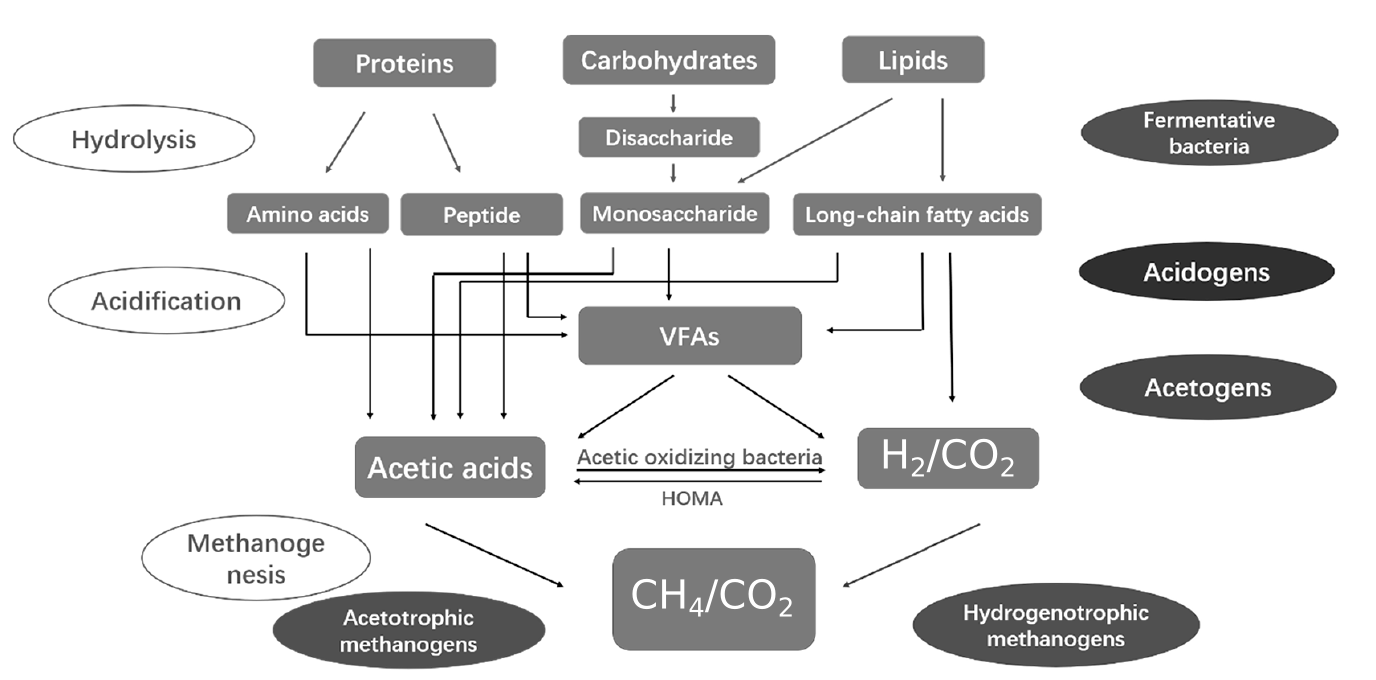
\includegraphics[width=\textwidth]{img1}

\caption[Schematic representation of anaerobic digestion]{Schematic representation of anaerobic digestion\citep{chen}}
\label{fg,ad}
\end{figure}


\subsubsection{Hydrolysis}

Organic biomass contain complex polymers which are inaccessible to microorganisms without being further broken down through hydrolysis. Hydrolysis breaks down large organic macromolecules to smaller components that can be utilized by acidogenic bacteria.
Hydrolytic bacteria are able to secrete extracellular enzymes that can convert carbohydrates, lipids, and proteins into sugars, \ac{LCFAs} and amino acids respectively. After enzymatic cleavage, the products of hydrolysis are taken up by acidogenic microorganisms. It is important to note that certain substrates, such as lignin, cellulose, and hemicellulose are difficult to degrade biologically due to their complex structures; enzymes are often added to enhance the hydrolysis of these carbohydrates\citep{patel}.

\autoref{tb,hydrolyticbacteria} shows substrates, products and characteristics of some typical hydrolytic bacteria.







\begin{table}
\center
\caption[Typical hydrolytic bacteria]{Typical hydrolytic bacteria.\citep{amani2010anaerobic}}


\vspace{0.3cm}

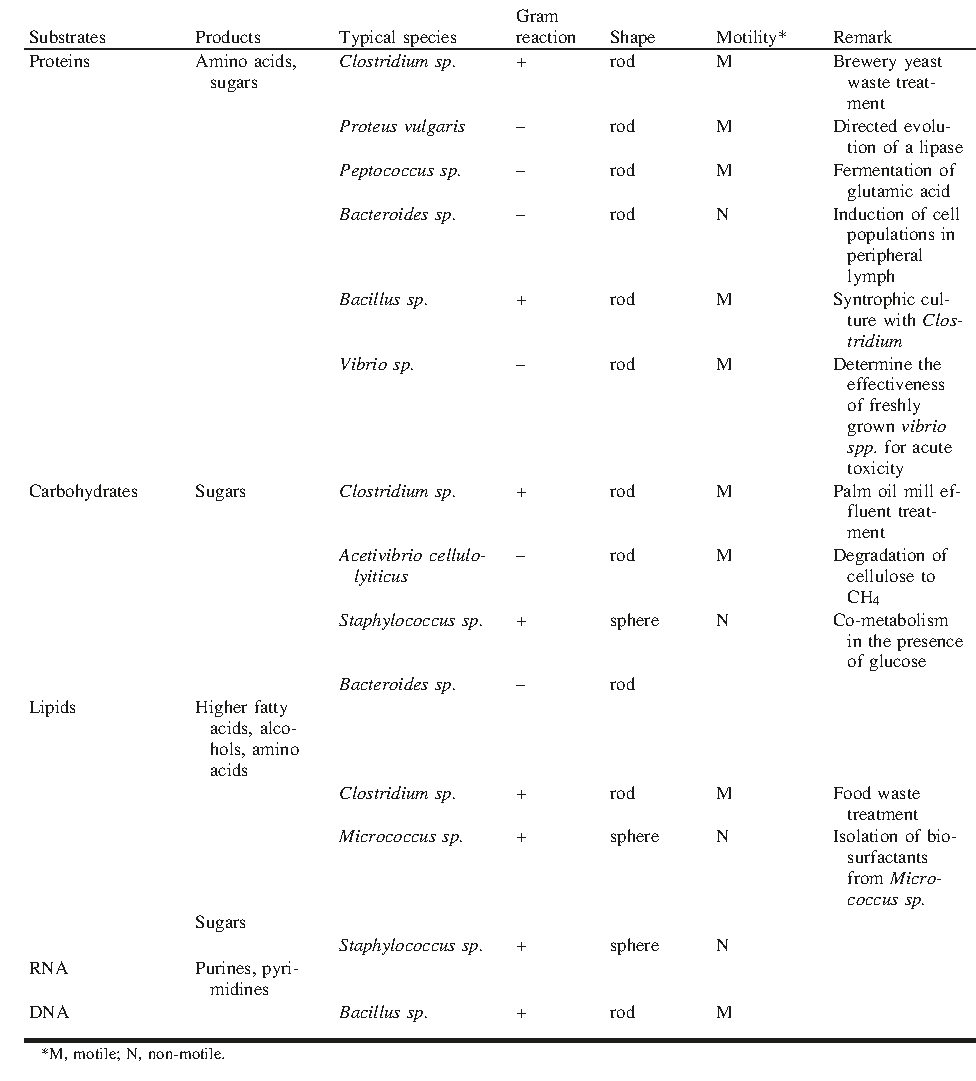
\includegraphics[scale=0.779]{hydrolyticbacteria}

\label{tb,hydrolyticbacteria}
\end{table}




 

\subsubsection{Acidogenesis}

By absorbing the products of hydrolysis through their cell membranes, acidogenic microorganisms are able to produce intermediate \ac{VFAs} and other products. \ac{VFAs} constitute a class of organic acids such as acetates, and larger organic acids such as propionate and butyrate\citep{patel}.


\autoref{tb,acidogenicbacteria} shows substrates, products and characteristics of some typical acidogenic bacteria.



\begin{table}
\center
\caption[Typical acidogenic bacteria]{Typical acidogenic bacteria.\citep{amani2010anaerobic}}
\vspace{0.3cm}
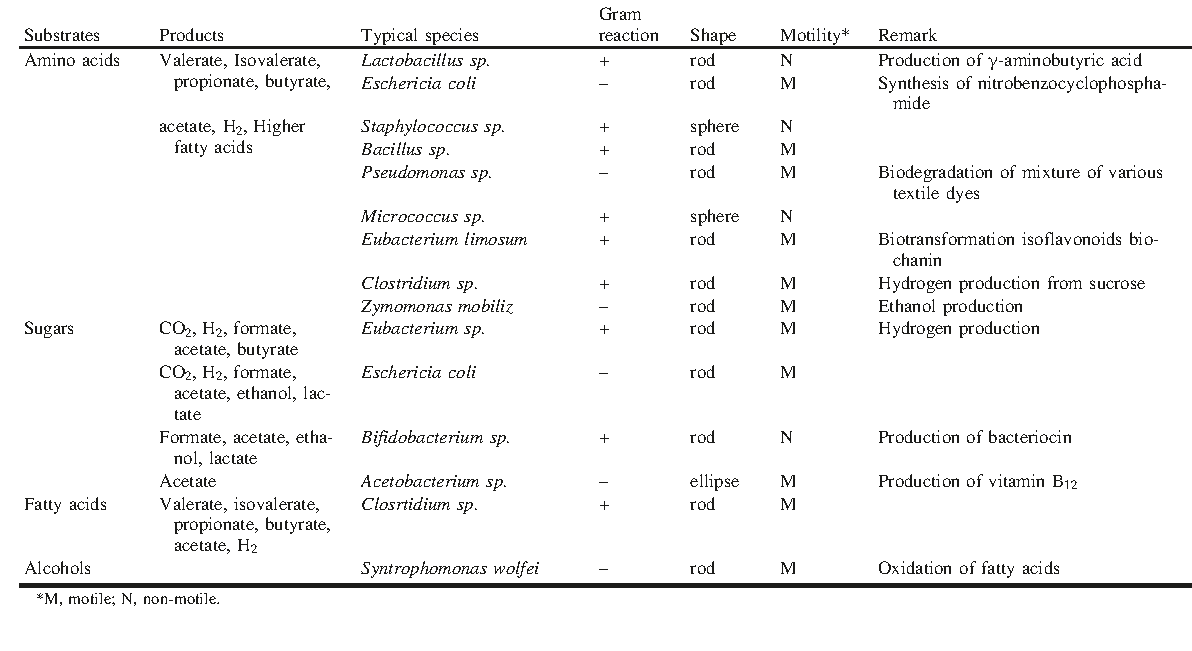
\includegraphics[scale=0.71]{acidogenicbacteria}
\label{tb,acidogenicbacteria}
\end{table}



\subsubsection{Acetogenesis}

With the production of acetate through acidogenesis, a portion of the original substrate has already been rendered into a substrate suitable for acetoclastic methanogenesis. However, other produced higher \ac{VFAs} have yet to be made accessible to methanogenic microorganisms. Acetogenesis is the process by which these higher \ac{VFAs}  and other intermediates are converted into acetate, with hydrogen also being produced. 


Excessive partial pressure of hydrogen proves to be deleterious to acetogenic microorganisms. However, due to the presence of hydrogenotrophic methanogens, hydrogen is able to be rapidly consumed while maintaining hydrogen partial pressures at a level favorable to acetogenesis. At the same time, lipids undergo a separate pathway of acetogenesis via acidogenesis and $\beta$-oxidation, where acidogenesis produces acetate from glycerol and $\beta$-oxidation produces acetate from \ac{LCFAs}\citep{patel}.

\autoref{tb,acetogenicbacteria} shows substrates, products and characteristics of some typical acetogenic bacteria.



\begin{table}
\center
\caption[Typical acetogenic bacteria]{Typical acetogenic bacteria.\citep{amani2010anaerobic}}
\vspace{0.3cm}
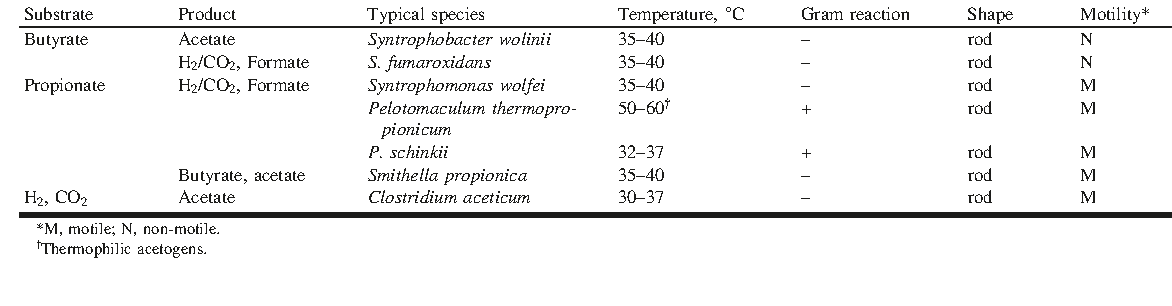
\includegraphics[scale=0.73]{acetogenicbacteria}
\label{tb,acetogenicbacteria}
\end{table}



\subsubsection{Methanogenesis}

Methanogenesis is the final stage of \ac{AD}. In this stage intermediates produced by previous stages of \ac{AD} are consumed by methanogenic archaea to produce methane\citep{patel}.

\autoref{tb,methanogenicarchaea} shows substrates, products and characteristics of some typical methanogenic archaea.



\begin{table}
\center
\caption[Typical methanogenic archaea]{Typical methanogenic archaea.\citep{amani2010anaerobic}}
\vspace{0.3cm}
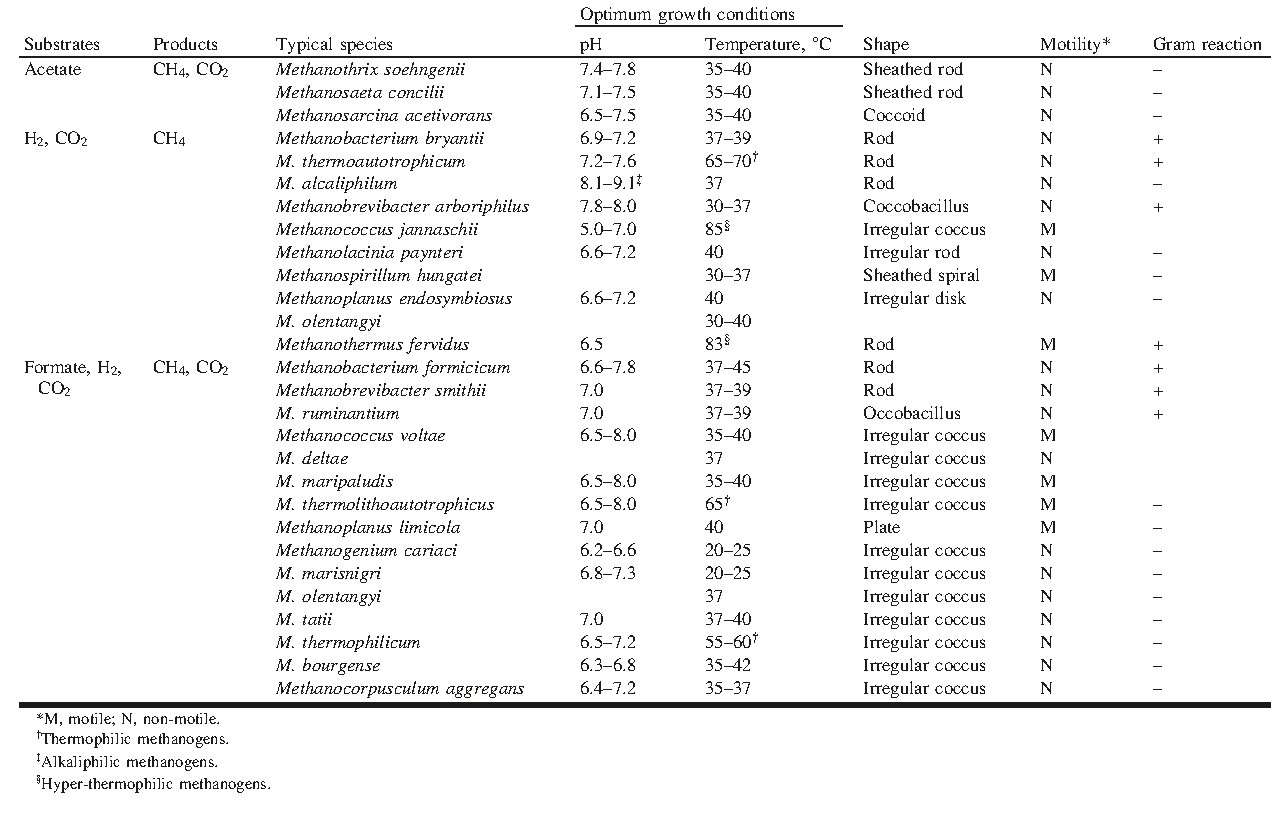
\includegraphics[scale=0.66]{methanogenicarchaea}
\label{tb,methanogenicarchaea}
\end{table}



\subsection{Syntrophy in methane production}

Syntrophy is a form of symbiosis of two metabolically different groups of bacteria, which enables degradation of various substrates\citep{zieminski2012methane}


Methanogenic archaea, which are involved in the production of methane exhibit synergistic relationships with Syntrophic bacteria. Syntrophic bacteria can't grow in form of pure cultures, but only when accompanied by microorganisms using hydrogen produced by them. Syntrophic interactions between bacteria and methanogens are the basis to maintain an \ac{AD} system working efficiently. These microorganisms, with distinct, but complementary metabolic capabilities, exchange electrons for energy purposes, normally through the transfer of small soluble chemical compounds, such as hydrogen or formate, that act as electron shuttles. This is called \ac{IET}.\citep{zieminski2012methane}

This interspecies hydrogen/formate transfer process is very important since the overall thermodynamics depends on the capacity of the microbial communities to maintain a low hydrogen partial pressure. Thus, diffusion limitations of these metabolites, between anaerobic bacteria and methanogenic archaea, can be important bottlenecks in the anaerobic conversion process.\citep{martins2018methane}





 





\subsection[Electron transfer mechanisms]{MECHANISMS OF \ac{IET} IN METHANOGENS}

 
   
   \acf{IET} can be classified into two types. Namely,
   
   \begin{enumerate}
   \item \ac{MIET}
   \item \ac{DIET}
   \end{enumerate}






\subsection[Mediated interspecies electron transfer]{\acf{MIET}}

\acf{MIET} is the most frequently described mode of \ac{IET}, whereby an electron carrying compound is transported by diffusion from mediator producing cells to mediator consuming cells along a concentration gradient. The mediator diffusion rate is limited by the concentration gradient at which oxidation and reduction reactions are thermodynamically feasible.\citep{storck2016modelling}. The following subsections briefly explain \ac{MIET} mechanisms.


\subsubsection{\ac{MIET} via Soluble Molecules}

 The most studied(in recent past) and widely known mechanism of electron transfer in methanogenic 
communities is the \ac{MIET} via hydrogen or 
formate. Syntrophic bacteria produce hydrogen or formate as a way
 to dissipate the reducing power, i.e., the electrons formed during the
  degradation of organic compounds and, in turn, methanogens utilize 
  those molecules as electron donors to reduce carbon dioxide to methane.
   Therefore, hydrogen/formate act as shuttles between hydrogen/formate forming bacteria
    and hydrogen/formate utilizing methanogens. At high hydrogen concentrations ($>$10 Pa),
     the hydrogenase activity is inhibited and consequently the metabolism of syntrophic bacteria is
      inhibited as well, while that of the methanogens is stimulated, and vice versa. Formate
       formation has been detected particularly in co-cultures growing on proteins or fatty acids 
       like propionate and butyrate. Under certain conditions, interspecies formate transfer
        may prevail because formate has a higher diffusion coefficient, comparing to hydrogen.
        Syntrophic interactions involving hydrogen or formate as electron shuttles are well described
         in co-cultures degrading common compounds formed during the \ac{AD} process such as butyrate, propionate, ethanol, and acetate \citep{martins2018methane}.
 
 
\subsubsection{\ac{MIET} via Extracellular Compounds}

 In numerous anaerobic environments, the interspecies electron transfer can also be 
mediated by insoluble compounds.
 Unlike soluble electron shuttles, such as hydrogen or formate, that can diffuse 
 in and out of the cell, insoluble compounds do not penetrate the cell surface.
  \citet{lovley1999humics} demonstrated that humus can mediate electron transfer 
  between humics-reducing and humics-oxidizing microorganisms. The 
  electron acceptor properties have been related mainly with the redox active quinone
   moieties present in humic substances. Several microorganisms were found to reduce 
   humic acids or anthraquinone-2,6-disulfonate \ac{AQDS} using hydrogen as electron donor 
   (e.g., the halorespiring bacterium, \textit{Desulfitobacterium} PCE1; the sulfate-reducing bacterium,
    \textit{Desulfovibrio} G11 and the methanogenic archaea, \textit{Methanospirillum hungatei} JF1) or 
    lactate (Desulfitobacterium dehalogenans and Desulfitobacterium PCE1).\citep{cervantes2002reduction, martins2018methane}
     Humus can also be reoxidized and act as an electron donor. For example, 
     humic acids can be redox mediators in the anaerobic substrate oxidation coupled 
     to the abiotic reduction of metal oxides such as Fe(III) and Mn(IV), 
     being reoxidized and participating in many cycles.\citep{cervantes2002reduction, martins2018methane}. Some bacteria of 
     the genus \textit{Geobacter} have been reported as quinone reducing microorganisms 
     using Fe(III) as the terminal electron acceptor but other microorganisms 
     share this ability, such as some \textit{Shewanella}, \textit{Desulfitobacterium}, \textit{Desulphuromonas, Geospirillum},   
     \textit{Wolinella}, and \textit{Geothrix}\citep{lovley1998humic} and the methanogenic archaea \textit{Methanopyrus kandleri}, \textit{Methanobacterium thermoautotrophicum}. The anaerobic oxidation of lactate and hydrogen by \textit{Desulfitobacterium dehalogenans} was obtained with \ac{AQDS} as mediator, associated with the reduction of goethite\citep{martins2018methane}.
     
     
\begin{figure}
\center
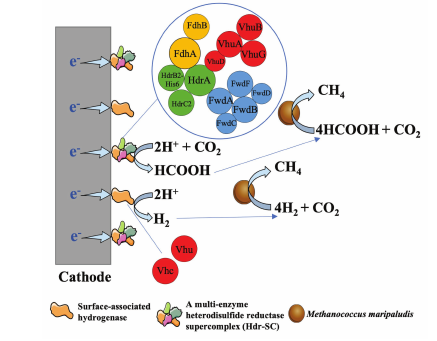
\includegraphics[scale=0.7]{miet}
\caption[Extracellular enzyme dependent MIET]{Extracellular enzyme dependent MIET\citep{gao2021putative}}
\label{fg,miet}
\end{figure}

 
\subsubsection{Extracellular enzyme dependent \ac{MIET}}


Hydrogenase and formte dehydrogenase can be released from the living or dead cells of \textit{Methanococcus maripaludis} and then are absorbed on the cathode surface. These surface-associated enzymes can catalyze the formation of hydrogen or formate, which are then rapidly consumed by \textit{M. maripaludis} cells to produce methane (\autoref{fg,miet})\citep{gao2021putative}.



\subsection[Direct interspecies electron transfer]{\acf{DIET}}


\acf{DIET} has been described in anaerobic environments, involving the 
formation of an electric current between electron-donating and electron-accepting
 microbes and without the need to produce and exchange 
 electron carriers (i.e., hydrogen and formate). DIET is analogous to direct 
 extracellular electron transfer, which consists in the electron transfer
  between cells and a solid-state electron acceptor such as iron and manganese 
  oxides or electrodes\citep{lovley2017syntrophy}. \autoref{fg,diet} shows proposed \ac{DIET} mechanisms.
  
  
  
\begin{figure}
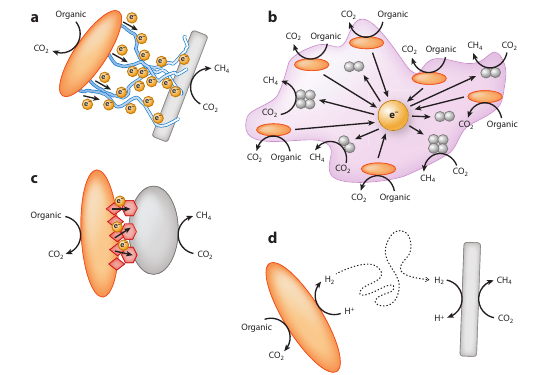
\includegraphics[scale=0.7]{diet}
\caption[Proposed DIET mechanisms]{Proposed DIET mechanisms\citep{lovley2017syntrophy}}
\label{fg,diet}
\end{figure}  
  
 
  \subsubsection[DIET promoted by e-pili]{\ac{DIET} promoted by \ac{e-pili}}
  
  
   \acf{DIET} is well studied
   in bacteria belonging to the genera \textit{Shewanella} and \textit{Geobacter}. \ac{DIET} was first
    described in defined co-cultures of \textit{Geobacter metallireducens}, an ethanol oxidizing bacteria,
     and \textit{Geobacter sulfurreducens}, a fumarate reducing bacteria. These microorganisms establish
      a syntrophic relationship, where \textit{G. metallireducens} metabolize the ethanol and the 
      \textit{G. sulfurreducens} reduces the fumarate. The ability of this culture for performing 
      \ac{DIET} was discovered when co-cultures formed with \textit{G. sulfurreducens} strains lacking the
       \textit{hyb} gene (thus unable to utilize hydrogen), were able to oxidize ethanol and to reduce fumarate.
        Under these conditions, interspecies electron exchange between \textit{G. metallireducens} and \textit{G. sulfurreducens }
        occurred directly via \ac{e-pili} and without the formation of soluble intermediates. \citet{rotaru2014new} showed that 
         \textit{Methanosaeta harundinacea}, a strictly acetoclastic methanogen, can receive electrons directly
          from \textit{G. metallireducens} to produce methane. The idea that \textit{Methanosaeta} species are acetoclastic 
          specialists, only producing methane from acetate, changed from this point on, since it seems to be 
          able to activate the carbon dioxide reduction pathway for methane production. In this context, the electrons 
          released by \textit{Geobacter} species are transferred, via \ac{e-pili}, directly to \textit{Methanosaeta}, but the cell machinery
           involved in electrons uptake by the methanogen is not yet known. These findings gave a new perspective on 
           the interspecies interactions taking place in anaerobic bioreactors producing methane \citep{martins2018methane}.


\subsubsection{\ac{DIET} promoted by conductive materials}

The presence of \ac{CM} such as \ac{GAC}, carbon cloth, and biochar appears to promote \ac{DIET}  via a conduction-based mechanism, 
in which electrons migrate through the \ac{CM} from electron- donating to electron-accepting cells.\citep{martins2018methane} Surprisingly,
 it was observed that the lack of pili and other cell component involved in the exogenous electron transfer can be 
 compensated by the presence of \ac{CM}, namely \ac{GAC}, carbon cloth and biochar.\citep{lovley2017syntrophy} This was verified in defined cocultures 
 of pilA-deficient strains of \textit{G. metallireducens} with \textit{Methanosarcina barkeri}, which could not convert ethanol to methane
  unless in the presence of \ac{CM}. This methanogenic co-culture in the presence of biochar were able to utilize 86\% 
  of the electrons released from ethanol oxidation for methane production, but without biochar no ethanol was 
  consumed and no methane was produced.\citep{chen2014promoting} Similarly, the lack of the \ac{OmcS},
   necessary for extracellular electron transfer in \textit{Geobacter} species, could be compensated by magnetite, 
   another conductive material. Without magnetite \textit{Geobacter} strains lacking genes for \ac{OmcS} were ineffective
    in forming viable co-cultures, but in the presence of magnetite, the \ac{OmcS} deficient mutants
     performed similarly to the wild type\citep{lovley2017syntrophy, martins2018methane}.
     
     
\subsubsection{\ac{DIET} promoted via outer cell surface}


The need for \acf{e-pili} or abiotic conductive materials to serve as interspecies electrical connectors may be alleviated if cells can form tight connections between their outer surfaces. This possibility is evident in co-cultures of \textit{Prosthecochloris aestuarii} and \textit{G. sulfurreducens}. \textit{P. aestuarii}, an anaerobic phototroph, directly accepted electrons from electrodes or \ac{DIET} to support photosynthesis. \textit{P. aestuarii} and \textit{G. sulfurreducens} formed tight associations with the two species in intimate contact\citep{lovley2017syntrophy}.


\subsubsection{Hydrogen and Formate \ac{IET} versus \ac{DIET}}

An interesting approach toward the clarification of the importance of \ac{DIET} in 
methanogenesis was presented by \citet{storck2016modelling} who proposed a 
mechanistic framework that enabled the direct assessment of the relative 
feasibility of \ac{DIET} and \ac{MIET} in a 
thermodynamically restricted syntrophic system (propionate conversion to acetate and methane), 
through mathematical modeling. They found that \ac{DIET} could be more favorable than hydrogen \ac{MIET},
 but substantially less favorable than formate \ac{MIET} (1 order of magnitude rate difference), 
 assuming a default parameter set based on literature data. The model results also suggested
  that DIET may be a thermodynamically more feasible alternative to \ac{MIET} for diverse communities 
  limited by diffusion, which is contrary to experimental observations where nanowire \ac{DIET} is 
  commonly observed in dense aggregates possibly indicating that co-evolution and 
  co-metabolism are more important than external limitations in the simulated system. 
  These authors also suggested that \ac{CM} reduce resistivity, and leave only activation losses, making long-range transport even more feasible \citep{martins2018methane}.









\section{Structure of Archaellum}

The archaellum is the swimming organelle in the domain Archaea. Unlike bacterial flagella, archaellum is distinct in terms of molecular composition, mode of action and is has much thinner filament (typically 10–14 nm in diameter)\citep{meshcheryakov2019high}. The following section will briefly explain the structure of archaellum proposed for \textit{Pyrococcus furiosus} by \citet{daum2017structure} 
but should be universal to all motile archaea, as the core of the archaellum machinery  is conserved throughout Crenarchaeal, Euryarchaeal and Thaumarchaeal lineages.







 Archaella are composed of a limited number of Fla proteins, most of which are encoded in a single Fla operon.\citep{meshcheryakov2019high} 

The filament is composed of similar subunits of FlaB3 protein in case of \textit{M. hungatei}. Each FlaB3 subunit comprises two domains: N-terminal a-helix and a C-terminal globular part, similar to that described for archaellins of \textit{P. furiosus} and \textit{Methanocaldococcus jannaschii} which have FlaB0 and FlaB1 respectively in their filament


\begin{figure}[h]
\center
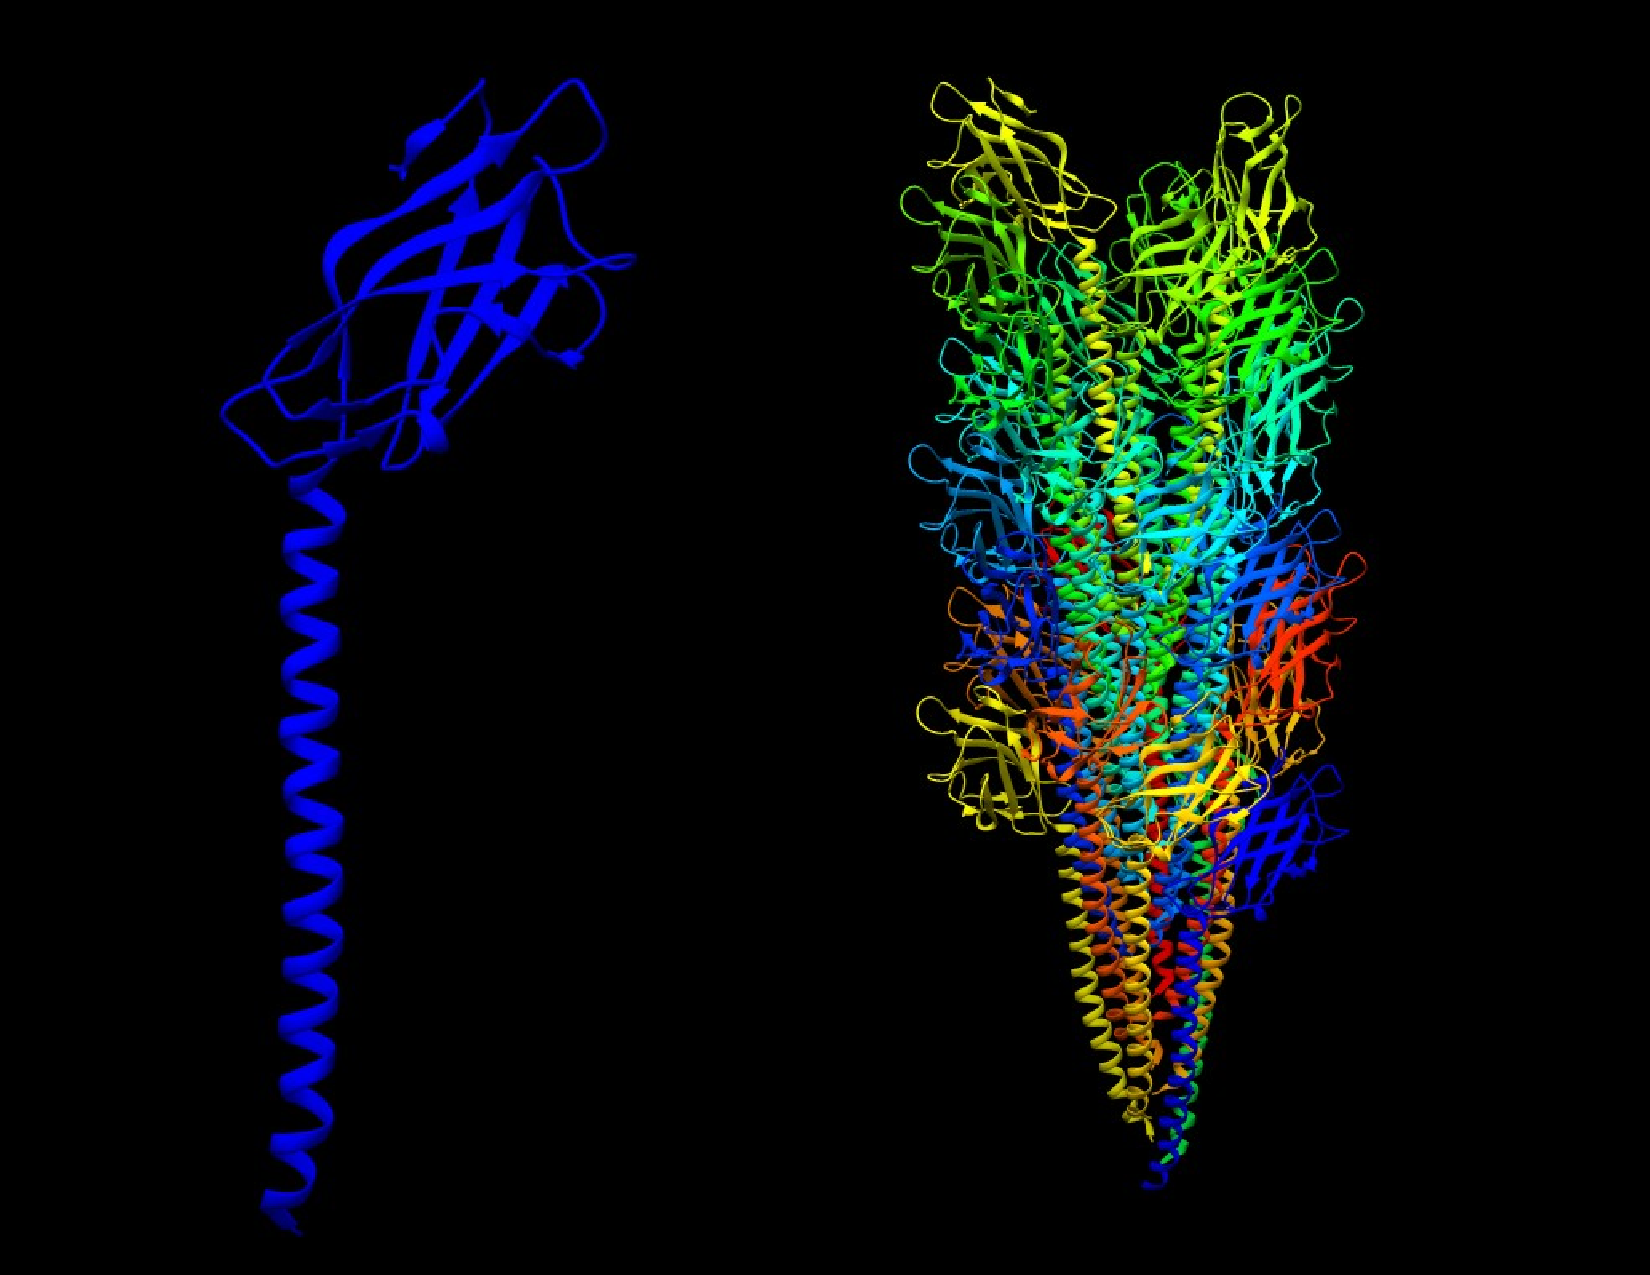
\includegraphics[scale=0.5]{subunit}
\caption{Archaellin subunit and filament}
\end{figure}




Archael filament crosses the S-layer and spans the periplasmic gap. They traverse the periplasm at variable angles of 60–90 degrees between the filament axis and the membrane plane. 


\begin{figure}[]
\center
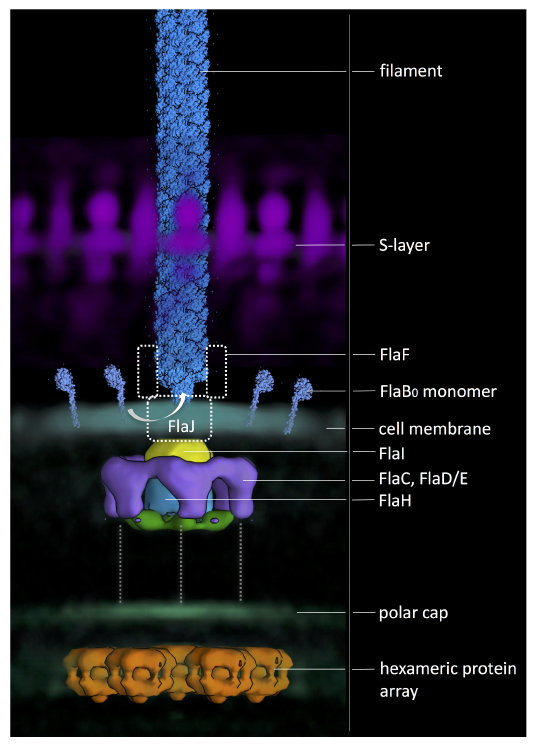
\includegraphics[scale=0.76]{archaellum}
\caption[Archaellum structure]{Archaellum structure\citep{daum2017structure}}
\end{figure}



These filaments emerge from a basal density on the cytoplasmic surface of the plasma membrane, which most likely corresponds to the archaellar motor.


Each of these densities is located in  gap between the membrane and a sheet-like cytoplasmic structure called polar cap. The polar cap appears to be a hallmark of motile Euryarchaeota, as it has also been observed in related species.. 



Filament assembly and rotation is powered by the archaellar motor, which is composed of the fully membrane-embedded FlaJ, a bell-shaped cytosolic complex of FlaI and FlaH and a surrounding cytosolic ring, most likely consisting of FlaC and D/E. In the periplasm, the filament is thought to be coordinated by FlaF.


The archaellar motors are juxtaposed to the polar cap, which in \textit{P. furiosus} is only present in combination with an archaellar bundle. This co-localisation indicates that archaella and polar cap are co-regulated and suggests a strong functional connection. It is conceivable that the polar cap functions in concentrating archaella at one cell pole and acts as an anchor to fix the motor complexes in the bilayer to prevent futile rotation. The polar cap is associated with protein complexes that form hexameric protein arrays. While the identity of these complexes is unknown, their localisation next to the archaellar motors suggests that they may be mechanistically linked to motor function.

The first steps of archaellum assembly comprise N- or O-glycosylation and removal of the positively charged N-terminal MAKKG signal peptide from membrane-bound FlaB0 monomers(for \textit{P. furiosus}). Loss of these positive charges primes the individual archaellins for transfer from the lipid bilayer into the growing filament, aided by the membrane protein FlaJ. This process is driven by the amphipathic surface of the individual archaellins and catalysed by ATP hydrolysis through FlaI.

\section{Possible industrial application of e-pili}

\vspace{0.5cm}

\subsubsection{Bioenergy} 


For production of highly efficient microbial fuel cells, electron transfer should occur through biofilms so that microorganisms which are away from the Cathode can recieve electrons from it and increase total current output. E-pili can be useful for such long-range electron transfers and improve overall efficiency of microbial fuel cells\citep{sure2016microbial}.


\vspace{0.5cm}

\subsubsection{Bioremediation}


 \textit{Shewanella} and \textit{Geobacter} have been extensively studied for bioremediation of heavy metals. Discovery of e-pili in these microorganisms has improved their potential in this field. It has been shown that e-pili can play an important role in bioremediation of a heavy metal like uranium \citep{cologgi2011extracellular, sure2016microbial}.

\vspace{0.5cm}

\subsubsection{Bioelectronics}



Researchers think that e-pili may allow us to develop instruments usable in water and moist environments\citep{malvankar2012microbial}. Additionally, \citet{leung2011bacterial} characterized \textit{Shewanella oneidensis} e-pili and showed that they have enough mechanical strength  to be used as a building block for construction of electronic devices\citep{sure2016microbial}.



\vspace{0.5cm}

\subsubsection{Potential target for pathogenic microorganisms }




E-pili have been found in pathogenic biofilms causing \ac{BRONJ}\footnote{Chronic condition of the oral cavity resulting in mucosal ulceration, exposure of underlying necrotic bone and ensuing secondary complications\citep{payne2017worry}} and supposed to play an important role in maintenance and survival of it. This discovery is very important considering the fact that various human pathogenic microorganisms like \textit{ Streptococcus pneumoniae} and \textit{Corynebacterium diphtheriae} produce pili which are actively involved in pathogenesis\citep{soriani2010relevance}. Exoelectrogens with e-pili play specific role in host immune response. It needs to be studied whether pili are conductive in different pathogenic bacteria and, if so, what role they play in pathogenesis. In the phenomenon called `bioelectric effect’, electrically stimulated pathogenic biofilms showed increased susceptibility to antibiotics and this may happen because of disruption of conductive filaments within them as a result of electrical stimulation\citep{wanger2013electrically}. The bioelectric effect also supports the hypothesis that e-pili may play an important role in maintenance of pathogenic biofilms. Thus, e-pili can be a potential target for prevention and treatment of certain diseases\citep{sure2016microbial}.






\section[Electrically conductive archaella of \textit{M. hungatei}]{Electrically conductive archaella of \textit{Methanospirillum hungatei}}

\textit{Methanospirillum hungatei} JF1 is a hydrogen and formate utilizing, methane producing archaeon and is the type species of the genus Methanospirillum, which belongs to the family Methanospirillaceae within the order Methanomicrobiales\citep{gunsalus2016complete}. In 1966, \citet{smith1966microbial} reported the isolation
of a new spiral-shaped methanogenic bacterium
from sewage sludge. \citet{ferry1974methanospirillum} in 1974 described the genus \textit{Methanospirillum} and the type species was named \textit{M. hungatii} and type strain \textit{M. hungatii} JF-1 (now \textit{M. hungatei} JF-1 \citep{balch1979methanogens}) in honour of Robert Edward Hungate\footnote{Pioneer of anaerobic microbial ecology. Developed the techniques for the culturing of anaerobic microbes\citep{chung1997robert}}.These archaea produce colonies that are yellow, circular, and convex with lobate margins; an optical
pattern of regular, light and dark striations throughout the colonies is the most
unique and distinguishing characteristic\citep{ferry1974methanospirillum}.


Its morphology is distinct from other methanogens with the ability to form long chains of cells (up to 100 $\mu$m in length), which are enclosed within a sheath-like structure, and terminal cells with polar flagella. The genome of \textit{M. hungatei} strain JF1 is the first completely sequenced genome of the family Methanospirillaceae, and it has a circular genome of 3,544,738 bp containing 3,239 protein coding and 68 RNA genes\citep{gunsalus2016complete}.




First atomic model of \textit{M. hungatei} archaella, based on the cryo electron microscopy was built by \citet{poweleit2016cryoem} at 3.4 Å resolution. Each archaellum contains $\approx$ 61,500 archaellin subunits organized into a curved helix with a diameter of 10 nm and average length of 10,000 nm. The tadpole-shaped archaellin monomer has two domains, a $\beta$-barrel domain and a long, mildly kinked $\alpha$-helix tail\citep{poweleit2016cryoem}.
The discovery of \ac{e-pili} begged the question if archaellum were conductive. In quest to answer this question, \citet{walker2019archaellum} chose \textit{M. hungatei} for their experiment since they were known to reduce extracellular electron acceptors and now thanks to \citet{poweleit2016cryoem}, the structure of archaellum was also available. Their experiment infact showed that the archaellum of \textit{M. hungatei} was conductive.


\vspace{0.3cm}
This led to questioning of the possibility that, electrically conductive archaellum may be a conduit for direct electron uptake by methanogens.





%----------------------------------------------------------------------------------------------------
%									Objectives
%----------------------------------------------------------------------------------------------------



\chapter{Objectives}


The purpose of this study is to find archaea with potential for \acf{DIET} through electrically conductive archaella by,

\begin{enumerate}
    \item Selection of proteins enabling direct electron transfer.
    \item Identification of microorganisms carrying analogues of selected proteins among organisms living in anaerobic ecosystems.

\item Analysis of potential protein analogues functionality based on sequence alignment.

\end{enumerate}







%----------------------------------------------------------------------------------------------------
%								Materials and Methods
%----------------------------------------------------------------------------------------------------

\chapter{Materials and Methods}

\section[Basic local alignment search tool(BLAST)]{\ac{BLAST}}

\ac{NCBI} Translated \ac{BLAST} web interface was used to find analogues of protein sequence of interest\citep{madden2003blast}. The last date of search was 07/09/2021. The search parameters used are in \autoref{blast}.

\begin{table}[h]
\caption{BLAST parameters}
\vspace{0.2cm}
\scriptsize
\centering
\begin{tabular}{l|l|l|l|l}
\hline
\multicolumn{2}{c|}{\textbf{General parameters}}                                    & \multicolumn{2}{c|}{\textbf{Scoring Parameters}}                                                                                                                  & \multicolumn{1}{c}{\textbf{Filters}}                                                                  \\ \hline
Expect threshold                                                        & 0.05      & Matrix                                                              & BLOSUM62                                                                                    & \multicolumn{1}{c}{\begin{tabular}[c]{@{}c@{}}Low complexity regions \\ filter selected\end{tabular}} \\ \hline
Word size                                                               & 2, 3 \& 6 & Gap Costs                                                           & Existence:11 Extension:1                                                                    &                                                                                                       \\ \hline
\begin{tabular}[c]{@{}l@{}}Max matches\\  in a query range\end{tabular} & 0         & \begin{tabular}[c]{@{}l@{}}Compositional\\ adjustments\end{tabular} & \begin{tabular}[c]{@{}l@{}}Conditional compositional\\ score matrix adjustment\end{tabular} &                                                                                                       \\ \hline
\end{tabular}
\label{blast}
\end{table}



\section{Clustal Omega}
 \acf{MSA} was performed using Clustal Omega tool on web interface provided by \ac{EMBL-EBI} using default settings\citep{madeira2019embl}.

\section{ESPript 3}

ESPript is a program which renders sequence similarities and secondary structure information from aligned sequences for analysis and publication purpose. It was used to visualize \ac{MSA} results\citep{robert2014deciphering}.

\section{SWISS-MODEL}

SWISS-MODEL
is a fully automated protein structure homology modelling server, accessible via the Expasy web server(Swiss institute of Bioinformatics). This was used to create models of archaella of methanogens found in this study whose protein structures were unavailable\citep{waterhouse2018swiss}.

\section{UCSF Chimera}

UCSF Chimera is a program for the interactive visualization and analysis of molecular structures and related data, including density maps, trajectories, and sequence alignments\citep{chimera}. This program (version 1.15) was used to visualize protein structures of the archaella. It was also used for hydrogenbond analaysis, analysis of protein surface property, analysis of clashes/contacts and superimposition of protein analogues.








%----------------------------------------------------------------------------------------------------
%									Results
%----------------------------------------------------------------------------------------------------


\chapter{Results}

\section{Translated BLAST}
Translated BLAST search using \textit{M. hungatei} JF-1 archaellum sequence was performed using three different word size parameter. With word size 3 and 6, no target organism was used while with word size 2, search was conducted against a list of methanogenic archae listed in \nameref{appendix} (page no. \pageref{appendix}). All word sizes revealed same result. The 34 methanogenic organisms found are listed in \autoref{tb,resultlist}. The organisms found had on average 30\% percentage identity match compared to sequence of \textit{M. hungatei} JF-1 with \textit{Methanospirillum sp} J.3.6-F.2.7.3 having highest percentage identity match(54.39\%). Most organisms had on average 3 copies of the gene with \textit{ Methanosphaerula palustris} E1-9c having the highest number of gene copies (8). Most of the organisms found were of genus \textit{Methanosarcina} (19 out of 34). Few non methanogenic archae were found to have \textit{M. hungatei} archaellum analogues. They are, \textit{Archaeoglobus fulgidus, Archaeoglobus profundus, Geoglobus acetivorans, Thermosphaera aggregans, Desulfurococcus amylolyticus} and \textit{Candidatus Nitrosotenuis aquarius}.



\begin{table}[]
\caption{List of methanogenic archaea found}
\vspace{0.3cm}
\begin{tabular}{clcc}
   & \textbf{List of methanogenic archaea}             & \textbf{\% Identity} & \textbf{No. of copies} \\
   \hline \\
1  & Methanospirillum sp. J.3.6.1-F.2.7.3 & 54.39\%                      & 4                         \\
2  & Methanospirillum hungatei GP1        & 49.14\%                      & 4                         \\
3  & Methanoculleus marisnigri JR1        & 35.83\%                      & 2                         \\
4  & Methanoculleus chikugoensis MG62     & 35.29\%                      & 2                         \\
5  & Methanolinea sp. EsbE                & 33.70\%                      & 1                         \\
6  & Methanocella conradii HZ254          & 33.54\%                      & 1                         \\
7  & Methanoculleus bourgensis MAB1       & 33.52\%                      & 2                         \\
8  & Methanosphaerula palustris E1-9c     & 30.98\%                      & 8                         \\
9  & Methanosarcina acetivorans C2A       & 30.96\%                      & 3                         \\
10 & Methanocella arvoryzae MRE50         & 30.81\%                      & 2                         \\
11 & Methanosarcina siciliae HI350        & 30.46\%                      & 3                         \\
12 & Methanococcoides burtonii DSM 6242   & 30.00\%                      & 2                         \\
13 & Methanosarcina horonobensis HB-1     & 29.95\%                      & 3                         \\
14 & Methanosarcina mazei LYC             & 29.57\%                      & 3                         \\
15 & Methanosarcina sp. MTP4              & 29.28\%                      & 2                         \\
16 & Methanoculleus bourgensis BA1        & 29.14\%                      & 4                         \\
17 & Methanoregula formicica SMSP         & 29.05\%                      & 4                         \\
18 & Methanosarcina siciliae T4/M         & 28.93\%                      & 3                         \\
19 & Methanosarcina siciliae C2J          & 28.93\%                      & 3                         \\
20 & Methanolacinia petrolearia DSM 11571 & 28.57\%                      & 6                         \\
21 & Methanoculleus bourgensis MS2T       & 28.16\%                      & 2                         \\
22 & Methanoregula boonei 6A8             & 27.60\%                      & 2                         \\
23 & Methanosarcina mazei Tuc01           & 27.22\%                      & 1                         \\
24 & Methanosarcina mazei SarPi           & 27.22\%                      & 3                         \\
25 & Methanosarcina mazei Goe1            & 27.22\%                      & 3                         \\
26 & Methanosarcina mazei WWM610          & 27.22\%                      & 2                         \\
27 & Methanosarcina mazei S-6             & 27.22\%                      & 3                         \\
28 & Methanosarcina mazei C16             & 27.22\%                      & 2                         \\
29 & Methanosarcina mazei JL01            & 27.22\%                      & 2                         \\
30 & Methanosarcina mazei zm-15           & 27.22\%                      & 2                         \\
31 & Methanosarcina mazei TMA             & 27.22\%                      & 2                         \\
32 & Methanosarcina lacustris Z-7289      & 25.99\%                      & 1                         \\
33 & Methanosarcina sp. WH1               & 24.43\%                      & 1                         \\
34 & Methanosarcina sp. WWM596            & 24.43\%                      & 1                        
\end{tabular}
\label{tb,resultlist}
\end{table}


\section{Multiple sequence alignment}
\ac{MSA} was performed on all methanogenic archae found using clustal omega. when there were multiple strains, type strain was chosen to be portrayed. (\autoref{fg,msa}).

It can be observed that the $\alpha$ - helix from N-terminal side is highly conserved. All the sequences have phenylalanine in position 1, 13 and 20 which have been proposed to be the main reason for electrical conductivity of \textit{M. hungatei} archaella. There is quite a bit of variance in sequences that form $\beta$ barrel on C-terminal side with few small regions being conserved.


\begin{figure}
\raggedright
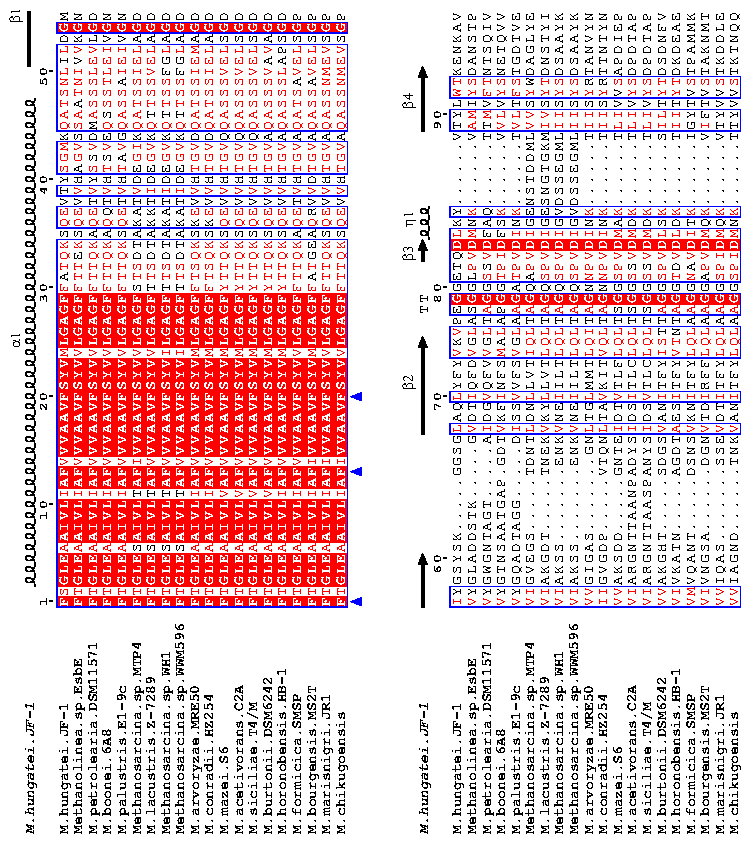
\includegraphics[scale=1.13]{alignment1}
\caption[Multiple sequence alignment (a)]{(a) Multiple sequence alignment}
Blue triangles indicate phenylalanine responsible for electrical conductivity 
\label{fg,msa}
\end{figure}






\begin{figure}
%\raggedright
\ContinuedFloat
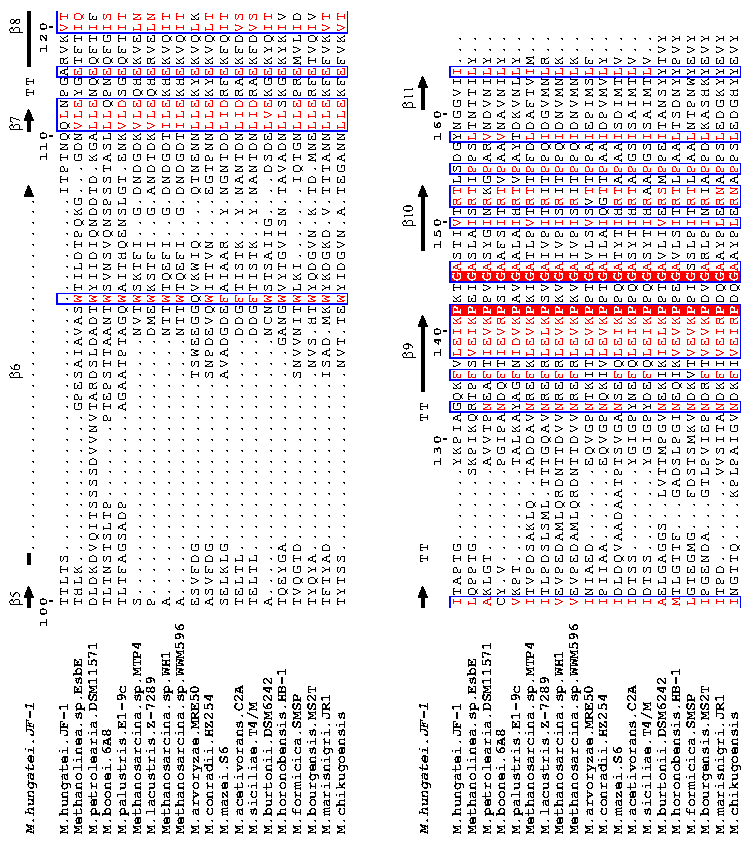
\includegraphics[scale=1.13]{alignment2}
\caption[Multiple sequence alignment (b)]{(b) Multiple sequence alignment}
\end{figure}





\begin{figure}
\center
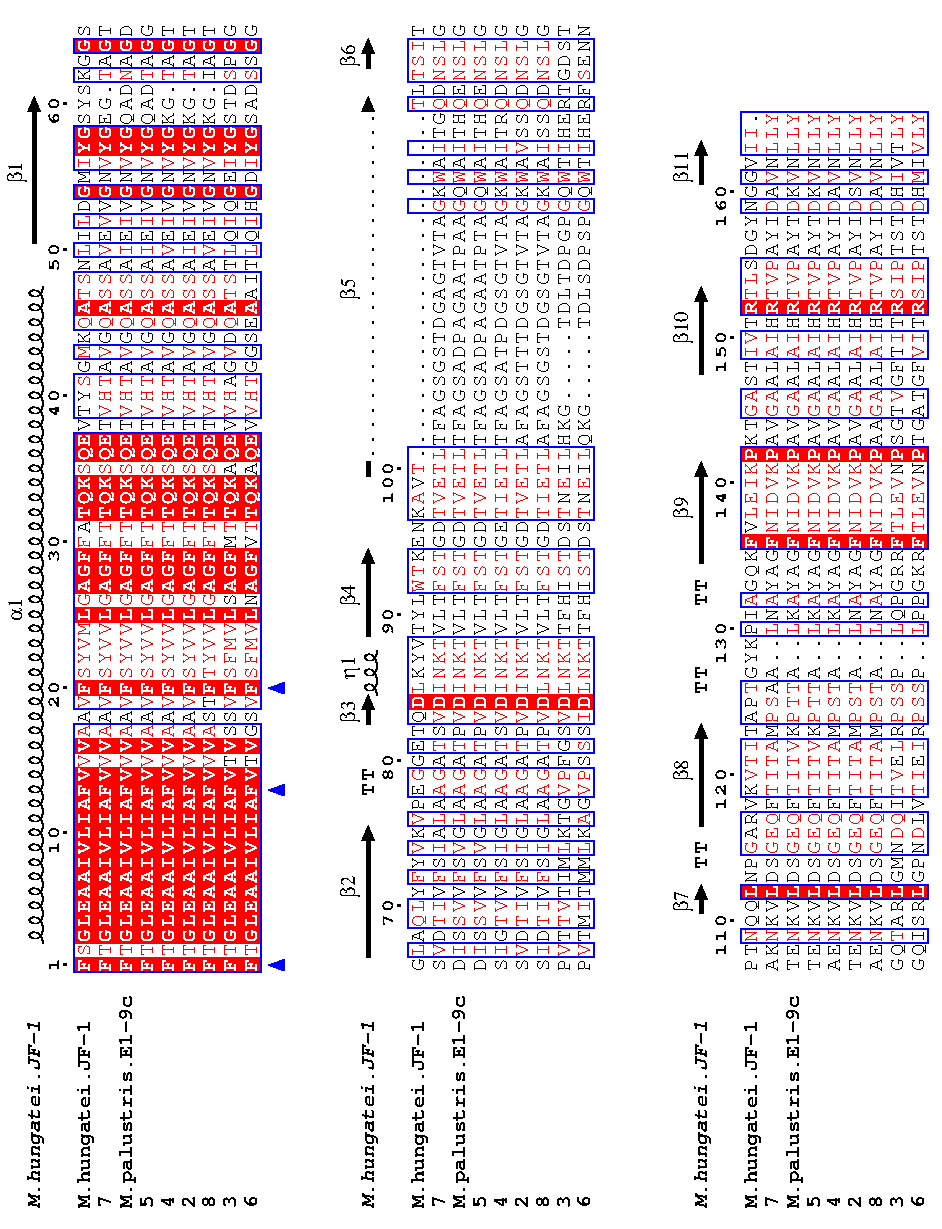
\includegraphics[scale=0.9]{alignment3}
\caption[Multiple sequence alignment of \textit{Methanosphaerula palustris}]{Multiple sequence alignment of \textit{Methanosphaerula palustris} E1-9c }
Sequences numbered in order of appearance in the genome.
\label{palustrismsa}
\end{figure}




\ac{MSA} was performed on all copies of archaellin genes in \textit{Methanosphaerula palustris} E1-9c in order to check if the copies are identical. \textit{M. palustris} was chosen since it had the most amount of copies. Interestingly, it yielded results similar to previous \ac{MSA} with $\alpha$ - helix being conserved and variability in $\beta$ barrels (\autoref{palustrismsa}). Two copies were more variable compared to others (3 and 6). More \ac{MSA} were performed with those two copies in order to find possibility of horizontal gene transfer but yielded no result. However, the search was limited so one can't rule out the possibility.


\section{Phylogenetic tree analysis}



Based on \ac{MSA} results, phylogentic tree was constructed (\autoref{ptree}) and compared with phylogentic tree constructed by \citet{adam2017growing} using bayesian phylogeny grounded on a 41 gene supermatrix. The 41 genes consist of 36 genes from the Phylosift marker genes list provided by \citet{darling2014phylosift}, plus RNA polymerase subunits A and B, and three universal ribosomal proteins (L7-L12, L30, S4) from \citet{liu2012control}. The tree is rooted according to \citet{raymann2015two} (\autoref{ptreeref}).



\begin{figure}[h]
\center
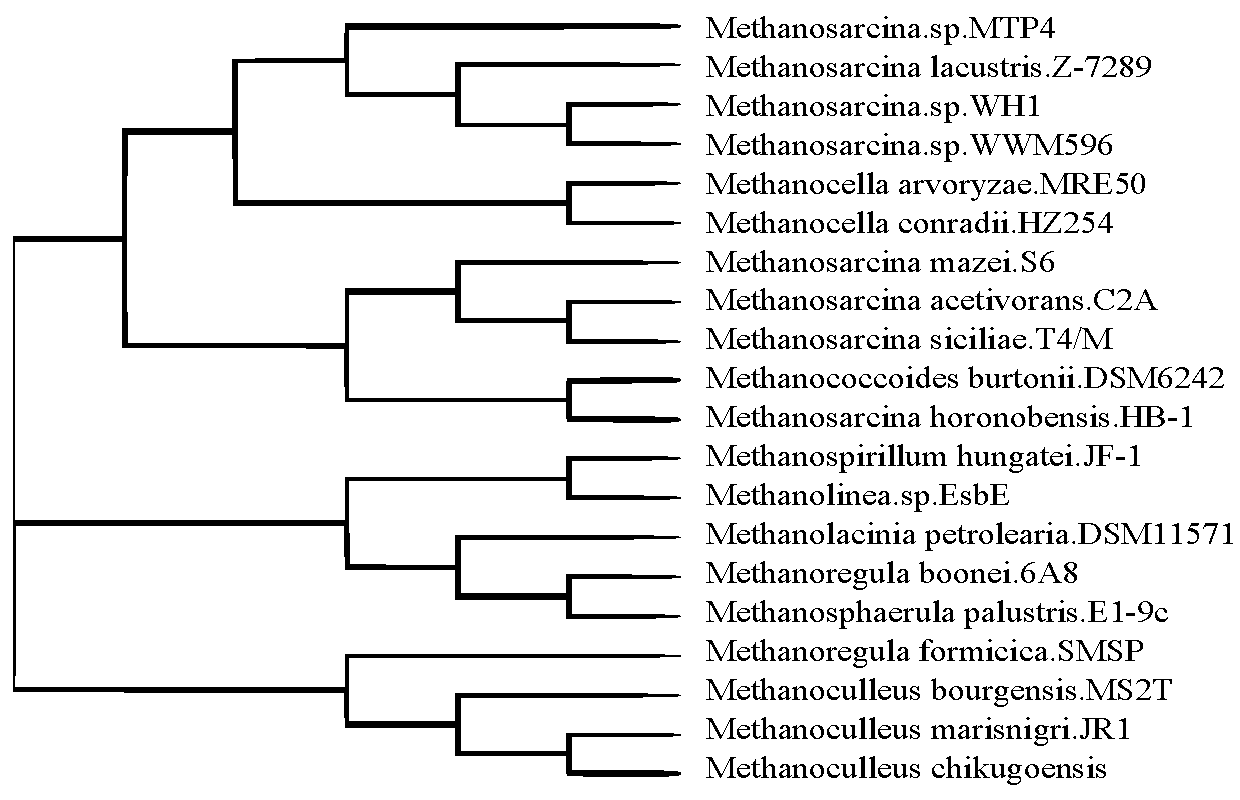
\includegraphics[scale=0.58]{tree}
\caption{Phylogenetic tree based on MSA}
\label{ptree}
\end{figure}

Phylogenetic tree constructed based on archaellin sequence and reference phylogenetic tree are similar.



\begin{figure}[]
\center
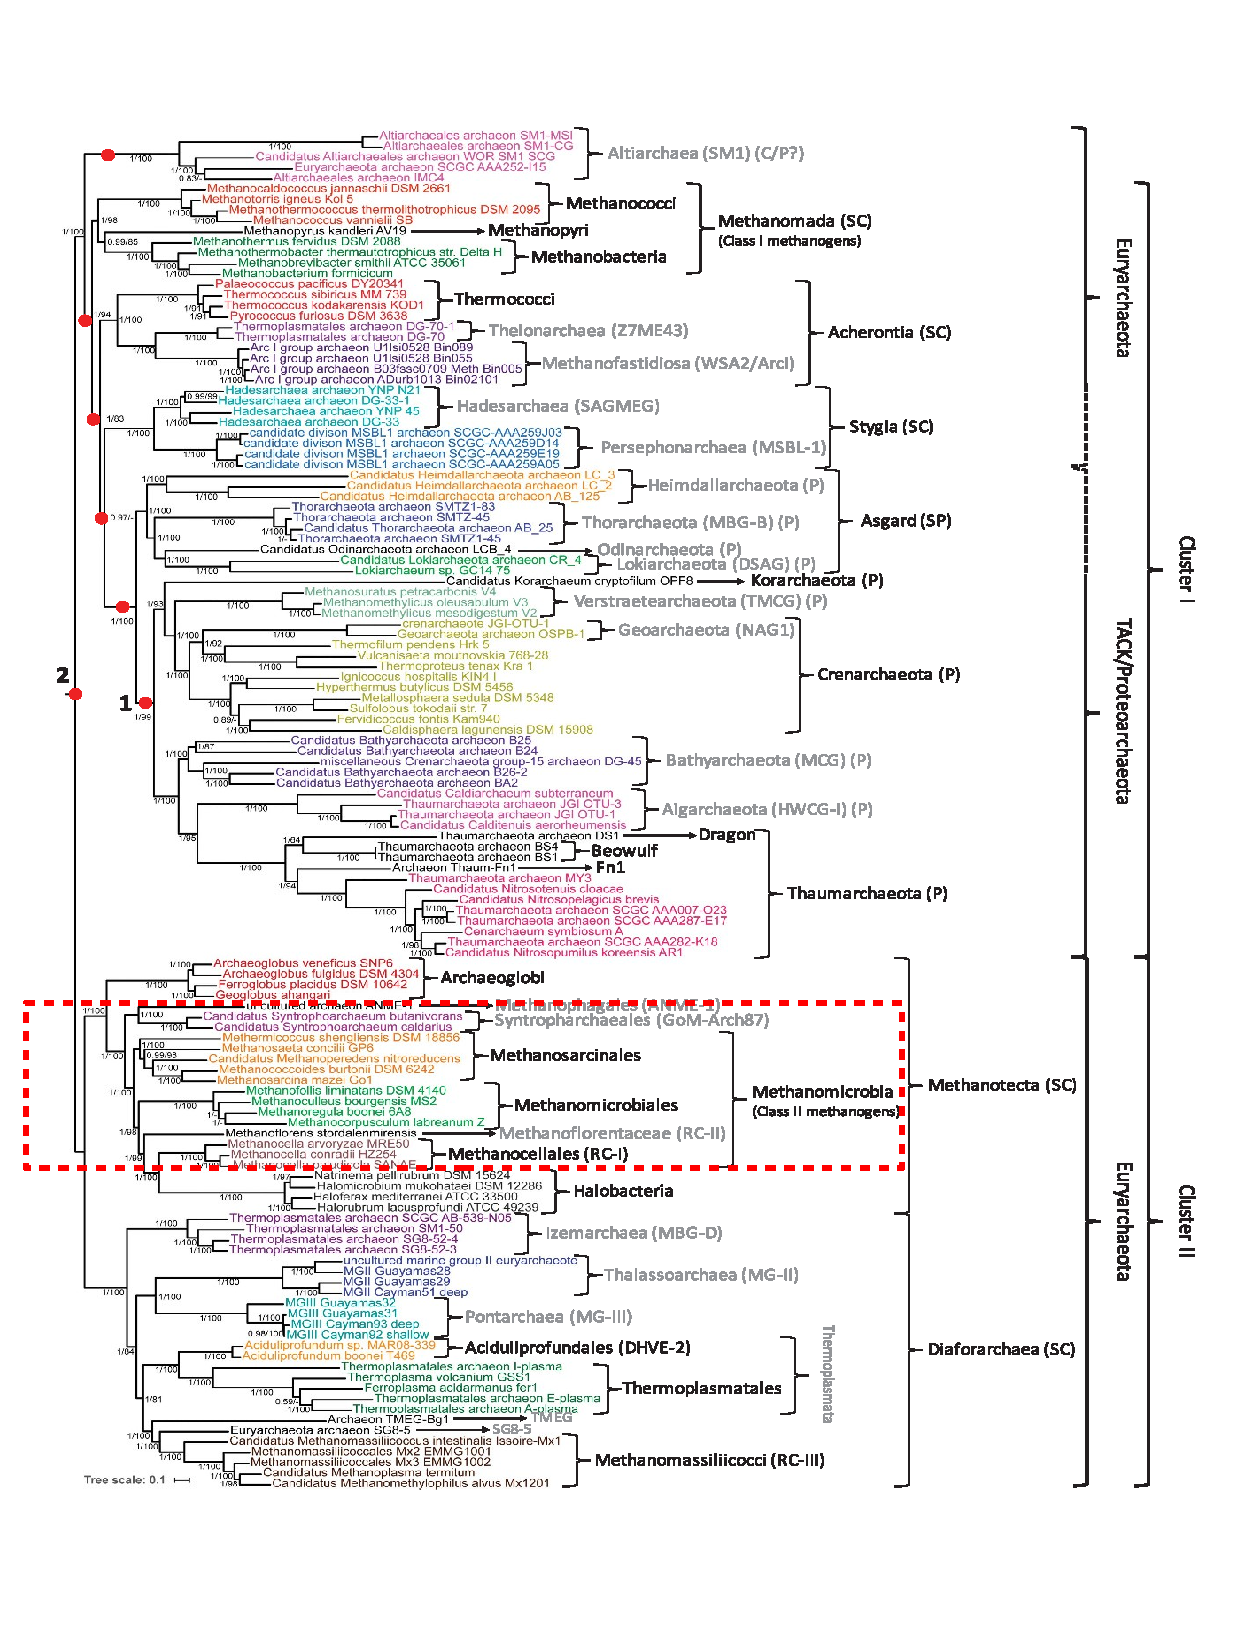
\includegraphics[scale=0.6]{tree2}
\caption[Reference phylogenetic tree]{Reference phylogenetic tree \citep{adam2017growing}}
\label{ptreeref}
\end{figure}





\begin{figure}[]
\ContinuedFloat
\center
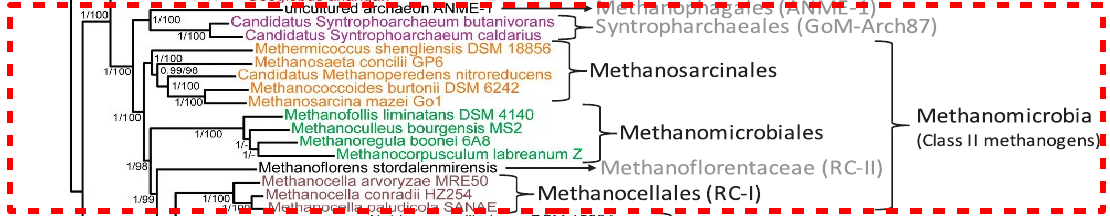
\includegraphics[scale=0.52]{tree3}
\caption*{}
\end{figure}


\section{Hydrogen bond analysis}

Hydrogen bond analysis was performed using chimera in hopes that it will shed some light on stability of archaella. Results revealed that the hydrogen bonds were mostly intra-subunit. Bonds between two subunits have been visualized in \autoref{hydrobond}. One can notice a single bond near the tip of $\alpha$ - helix.




\begin{figure}[h]
\center
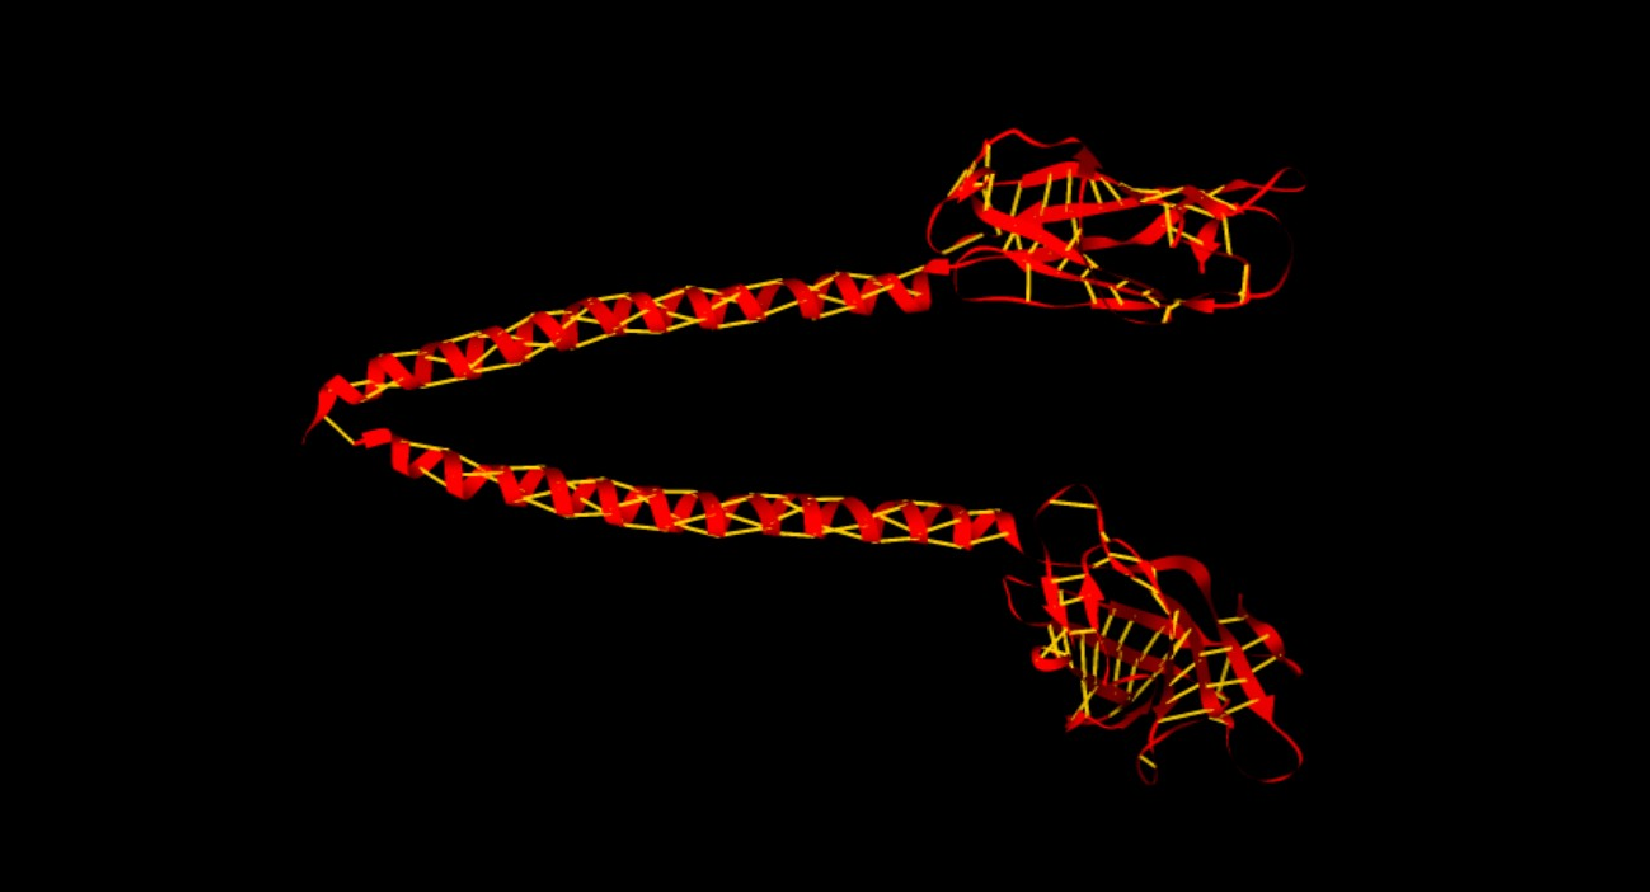
\includegraphics[width=0.8\linewidth]{hydrobond}
\caption{Hydrogen bond visualization}
Hydrogen bonds coloured in yellow
\label{hydrobond}
\end{figure}




\section{Protein surface property analysis}

In further attempt to understand reasons behind archaella stability, protein surface hydrophilic-hydrophobic property was visualized using chimera (\autoref{hydrophobicity}). Results revealed a hydrophobic $\alpha$ - helix which forms the core of the archaella and hydrophilic $\beta$ barrel which forms the external surface.

\begin{figure}[]
\center
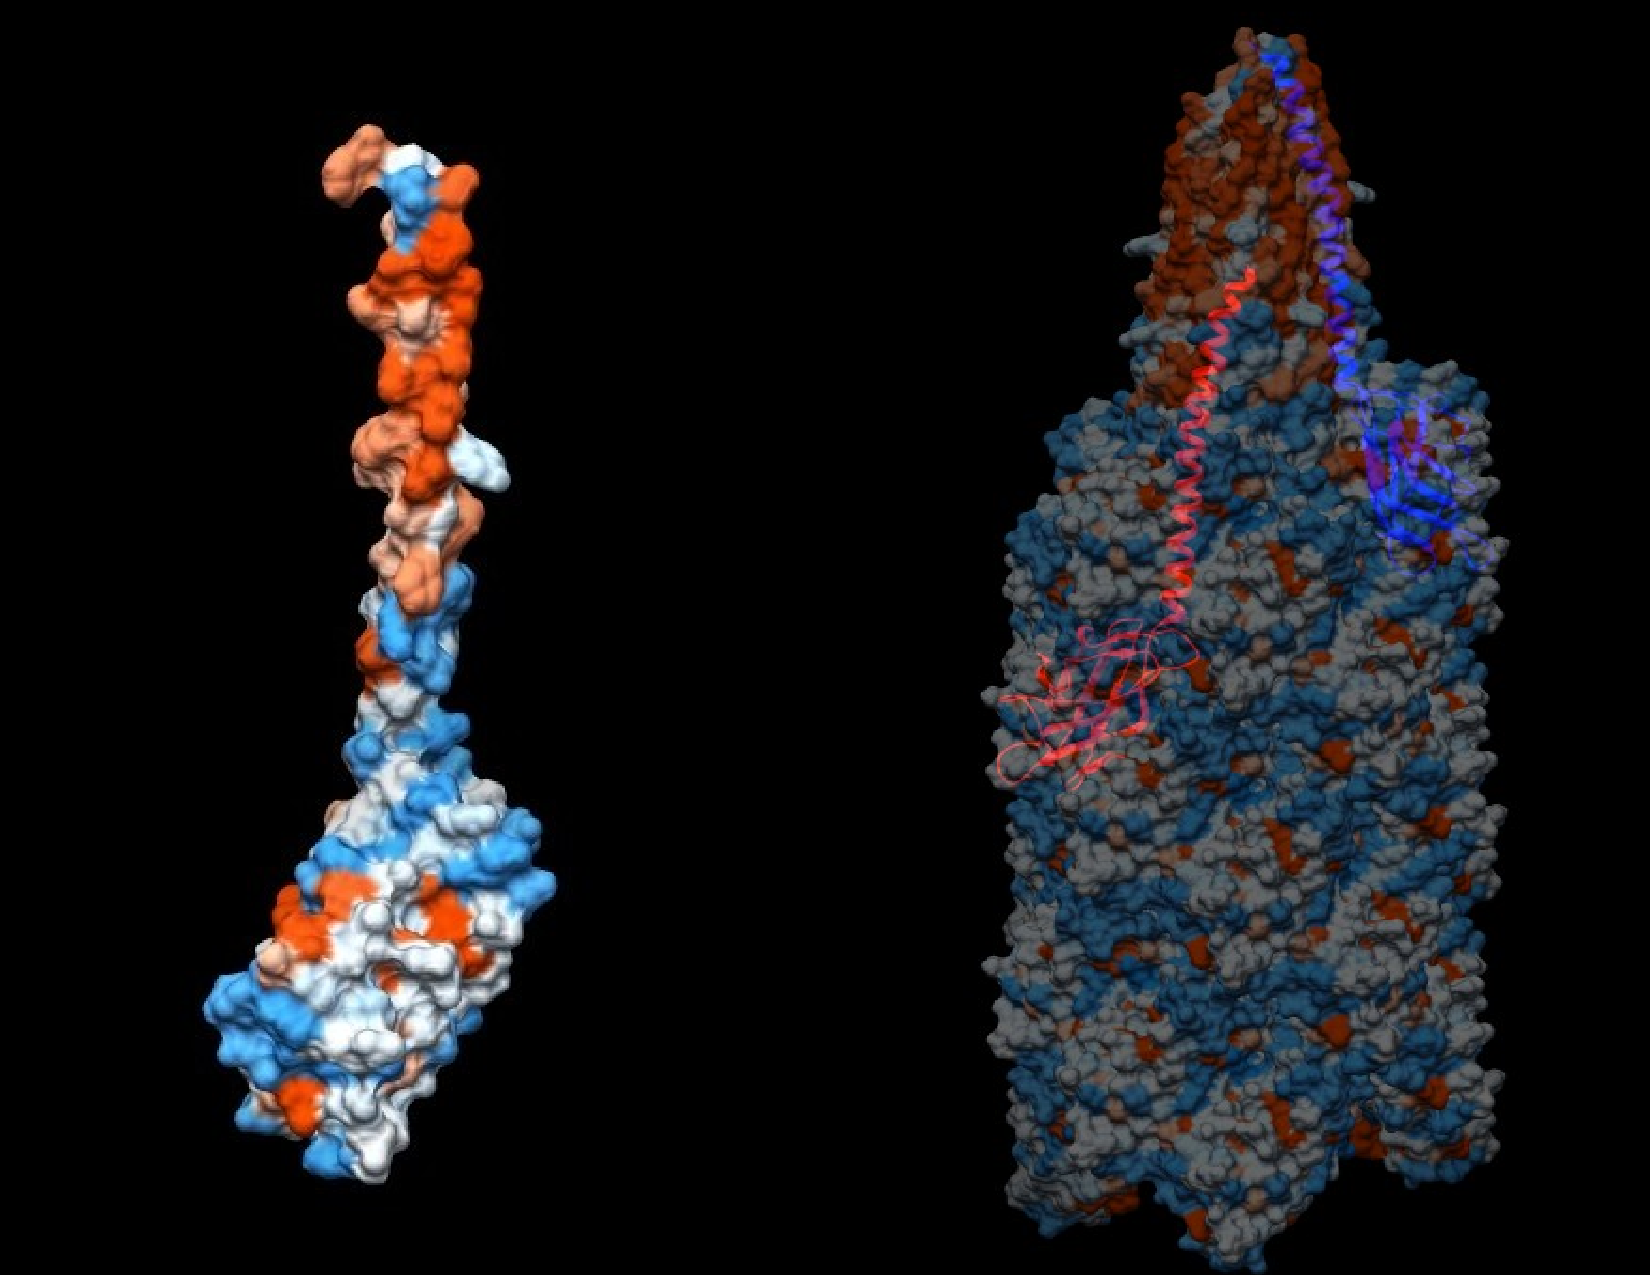
\includegraphics[width=0.85\linewidth]{hydro}
\caption{Hydrophobicity of protein surface}
Single subunit on left
\label{hydrophobicity}
\end{figure}



\begin{figure}[h]
\center
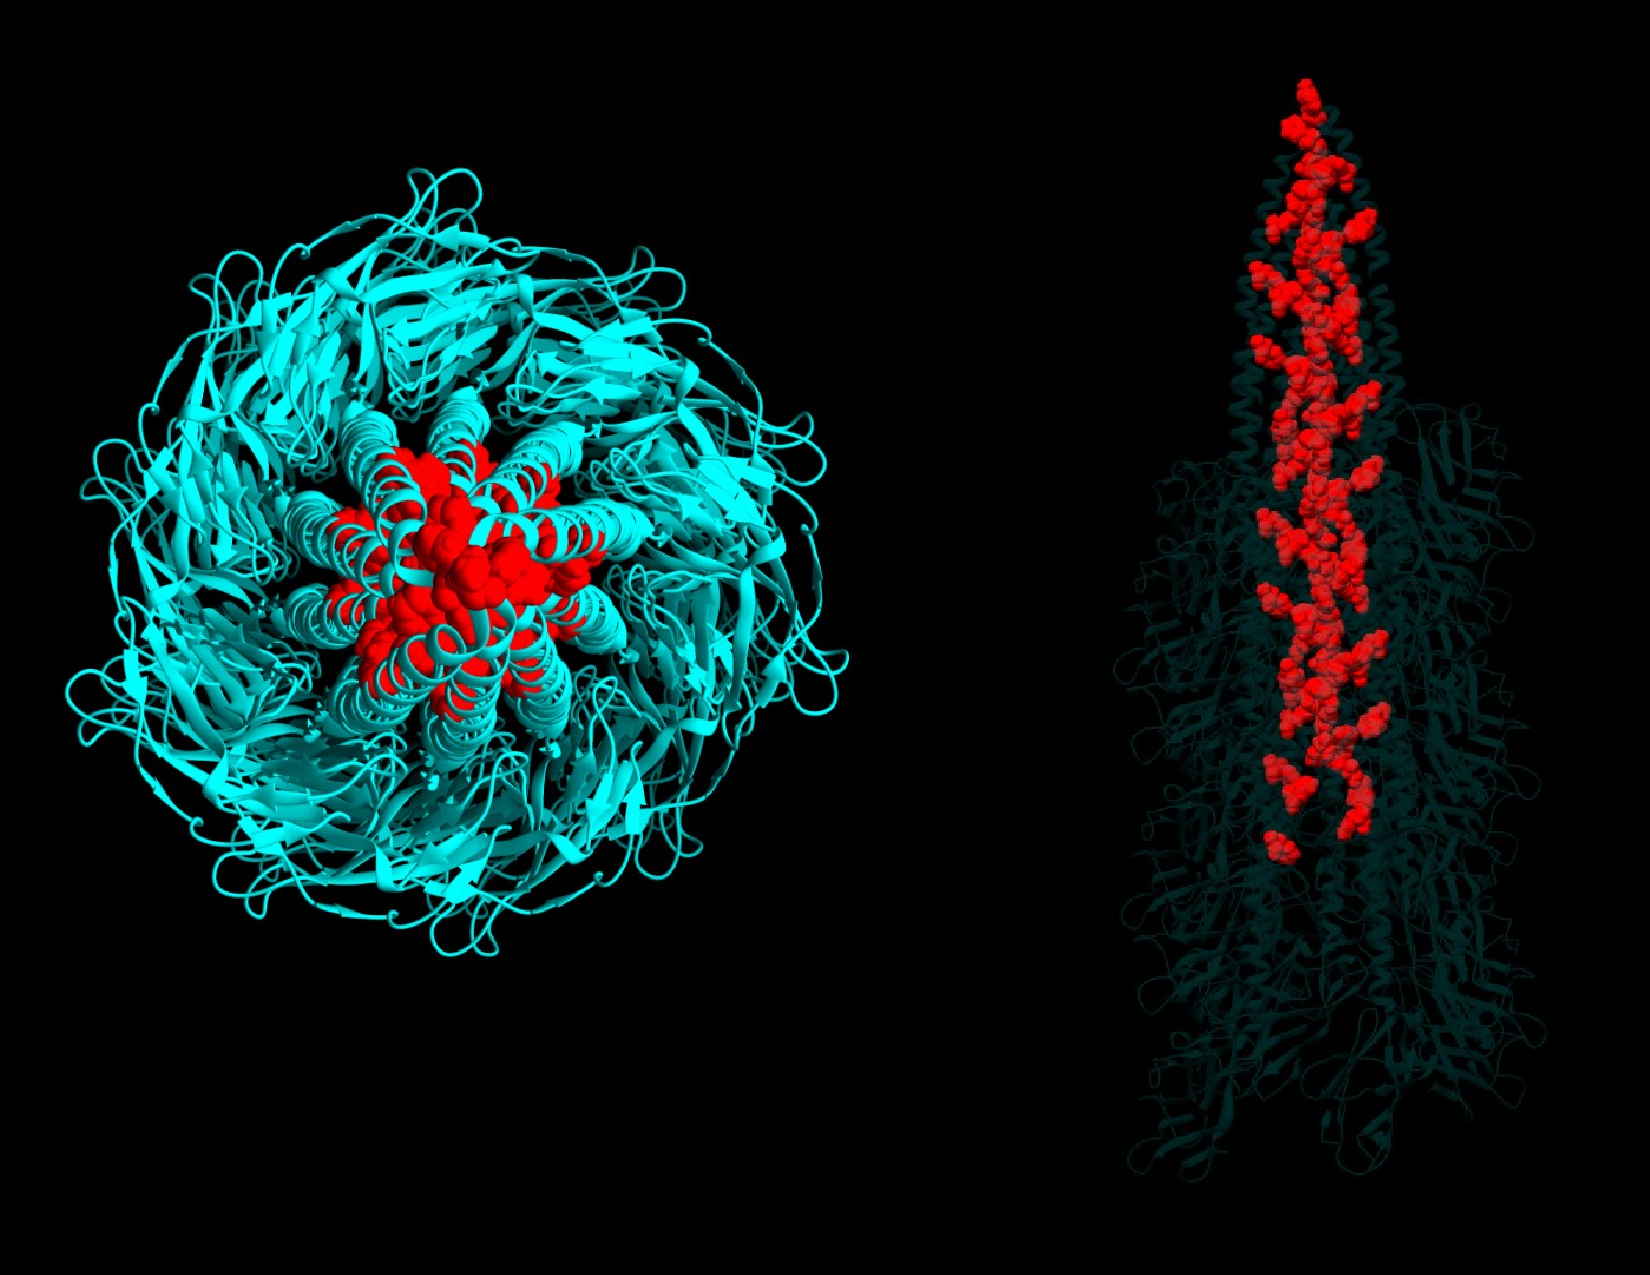
\includegraphics[width=0.85\linewidth]{overlap}
\caption{Phenylalanine visualization}
\label{overlaps}
\end{figure}


\section{Phenylalanine overlaps}

Clashes/contacts were analysed using chimera to study proximity of phenylalanine in archaella structure of \textit{M. hungatei}. The results showed clashes/contacts between phenylalanine from different subunits of the archaellum filament. The phenylalanine in these subunits were individually visualized. They form a christmas tree like structure, tightly packed in the core of the archaellum shown in \autoref{overlaps}. 



\clearpage

\section{Homology based modelling}

Since there were no structures available for the methanogens found in this study, homology based structural modelling was done using swiss-model. The models were analysed using chimera to check possibility of these organisms to form an archaella. Individual subunits were superimposed onto structure of \textit{M. hungatei} to see the similarity (\autoref{superposition}) and all the previous mentioned analysis were done. Based on this it could be deduced that the probability of these organisms to form a stable archaella is high. \autoref{homology} shows models built using swiss-model with individual subunit superimposed with \textit{M. hungatei}. The models portrayed were chosen based on their position in phylogenetic tree (\autoref{ptree}; Page no. \pageref{ptree}) for diversity.

\begin{figure}[]
\center
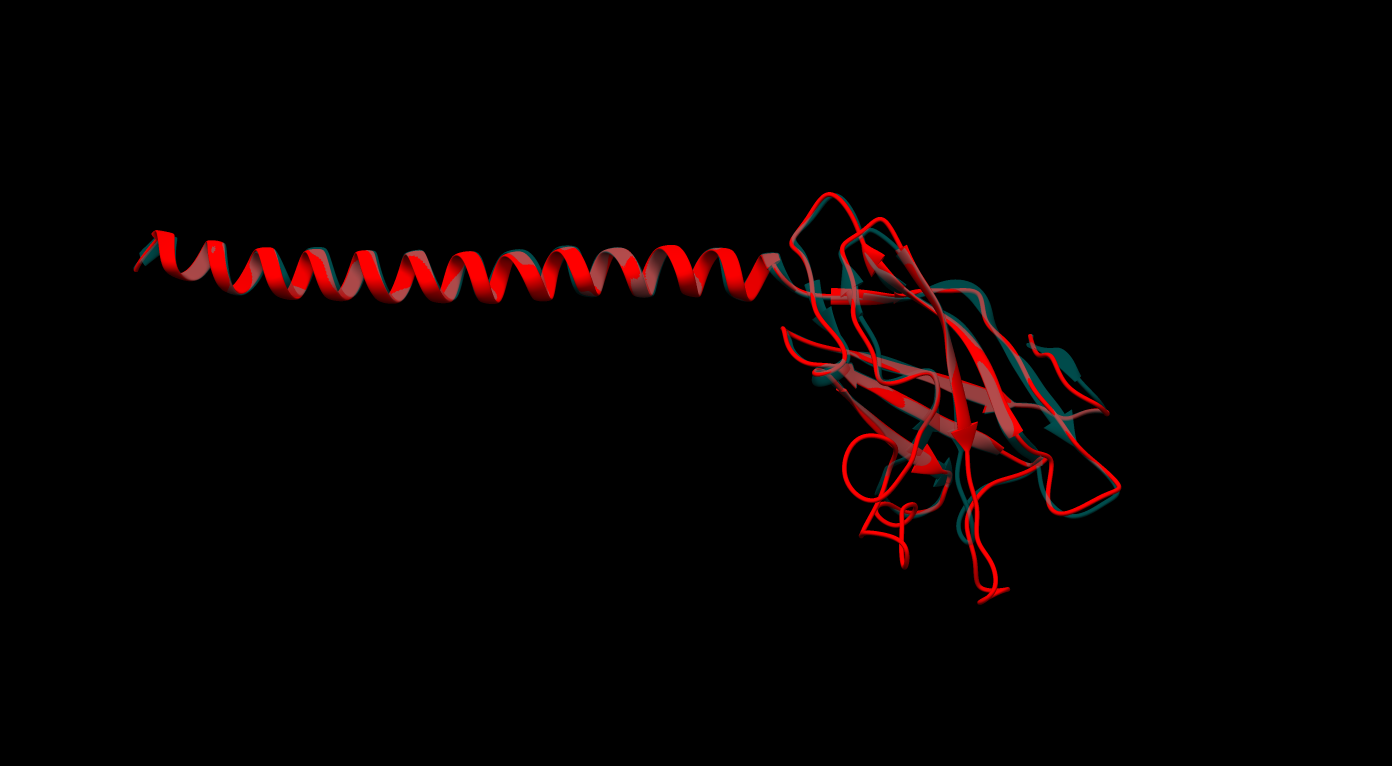
\includegraphics[width=1\linewidth]{superposition}
\caption{Superposition of individual subunit}
of \textit{M. hungatei} and \textit{Methanosarcina mazei}
\label{superposition}
\end{figure}







\begin{figure}
\begin{subfigure}{.5\textwidth}
  \centering
  % include first image
  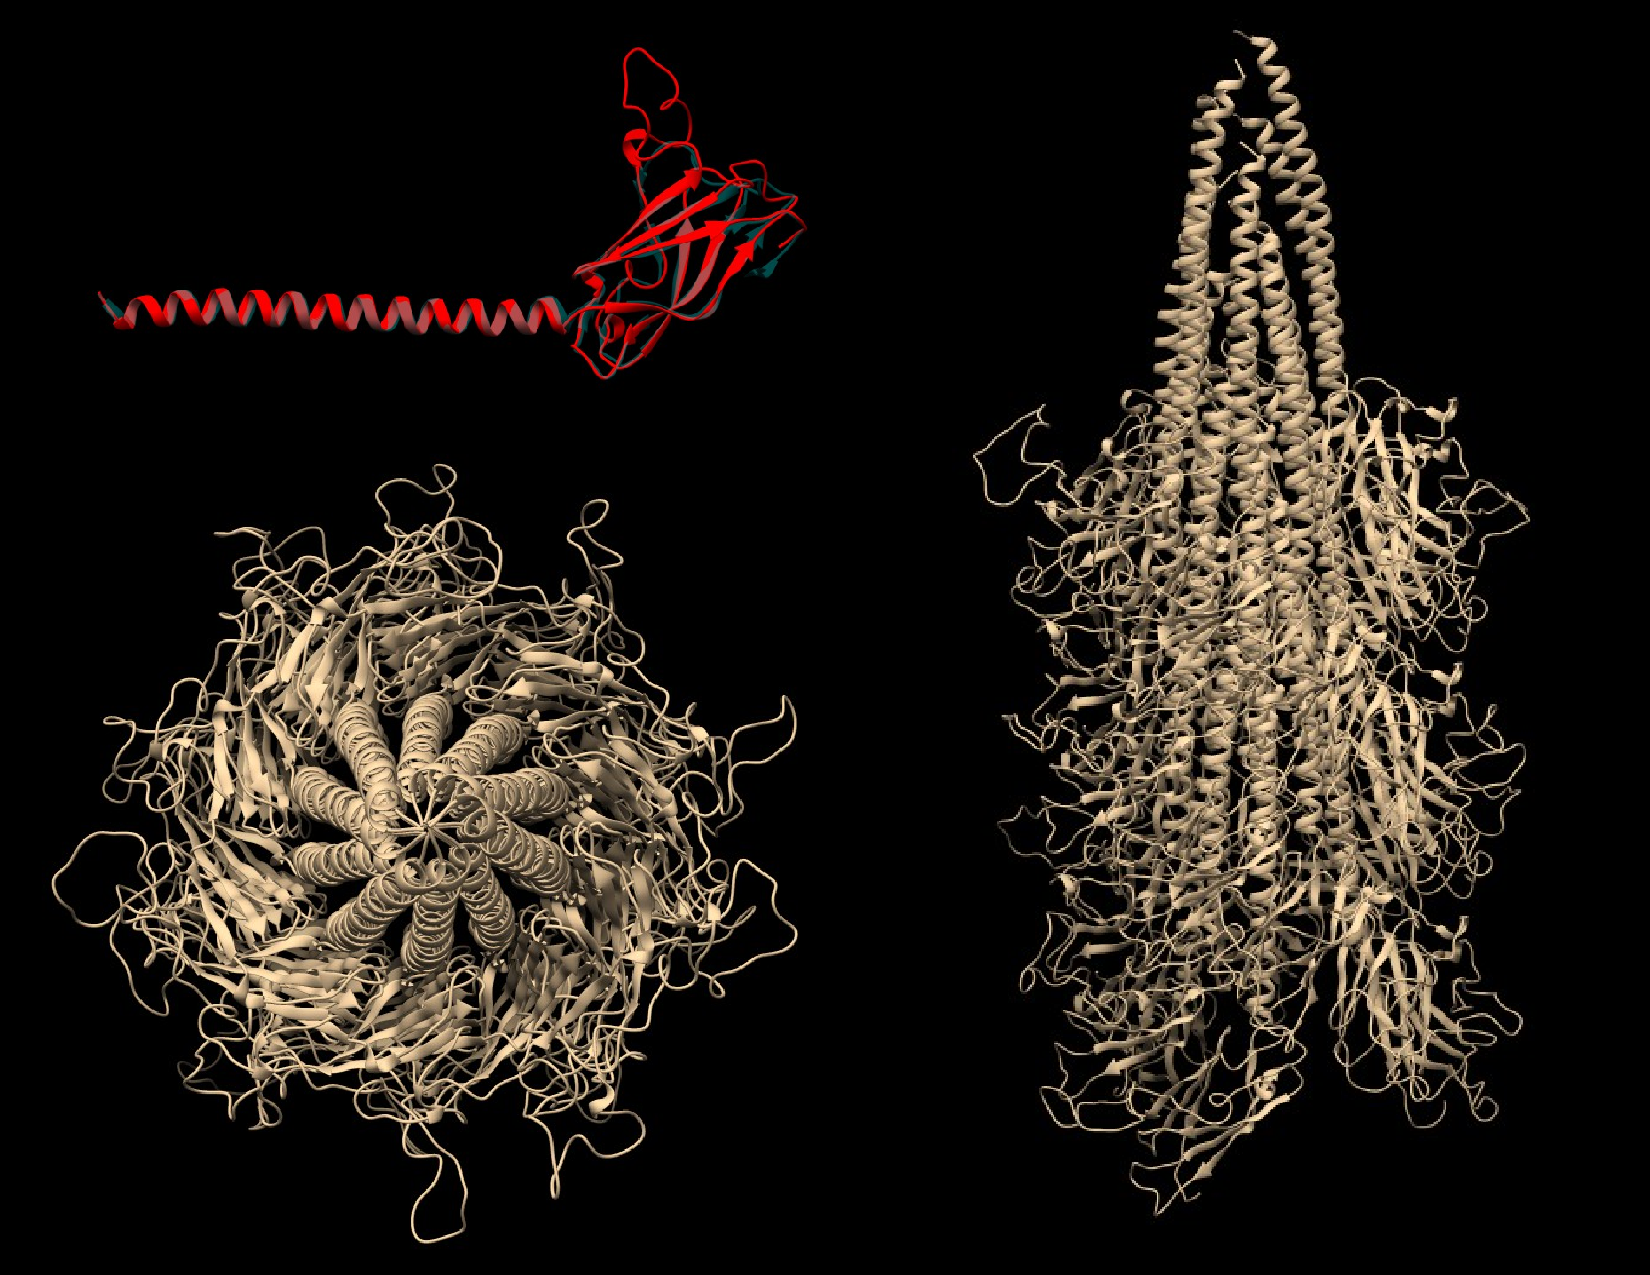
\includegraphics[width=0.9\linewidth]{boonei}  
  \caption{\textit{Methanoregula boonei}}
  
\end{subfigure}
\begin{subfigure}{.5\textwidth}
  \centering
  % include second image
  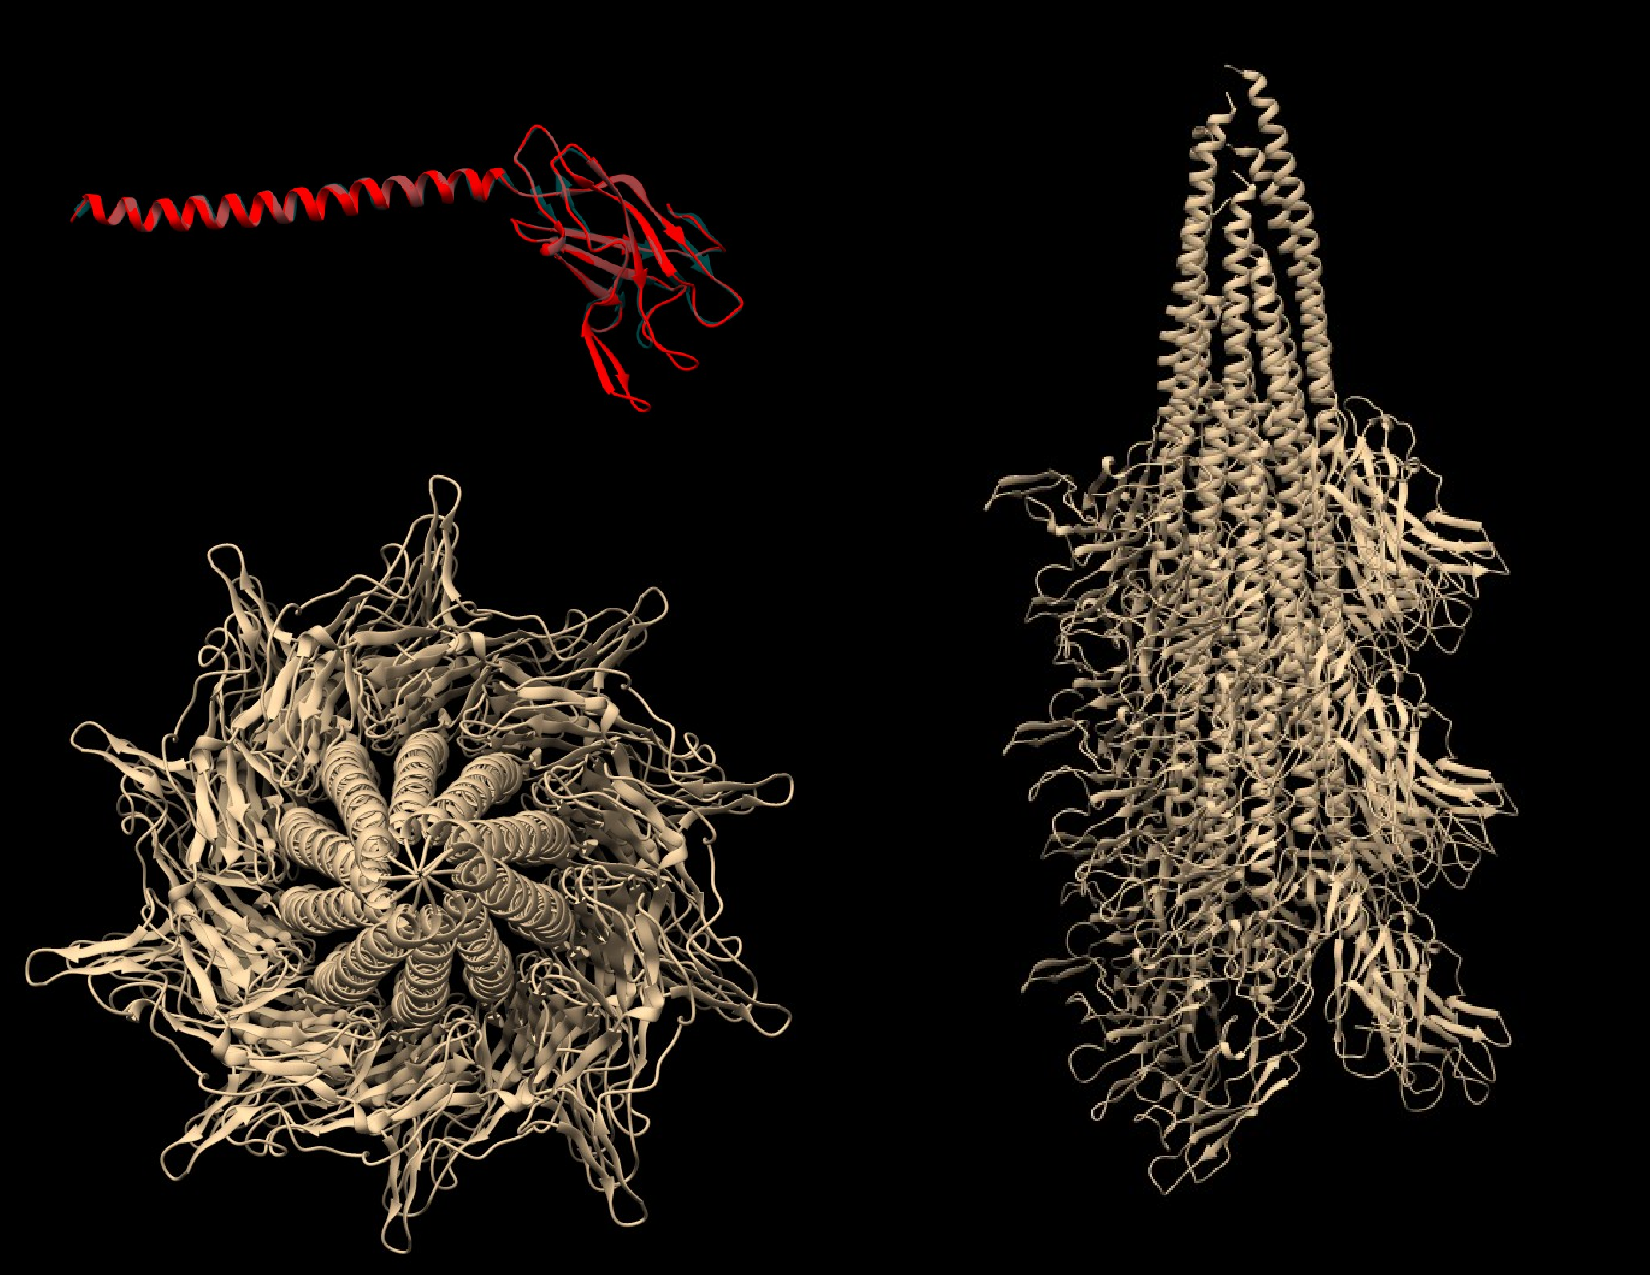
\includegraphics[width=.9\linewidth]{formicia}  
  \caption{\textit{Methanoregula formicia}}
  
\end{subfigure}

\vspace{0.3cm}

\begin{subfigure}{.5\textwidth}
  \centering
  % include third image
  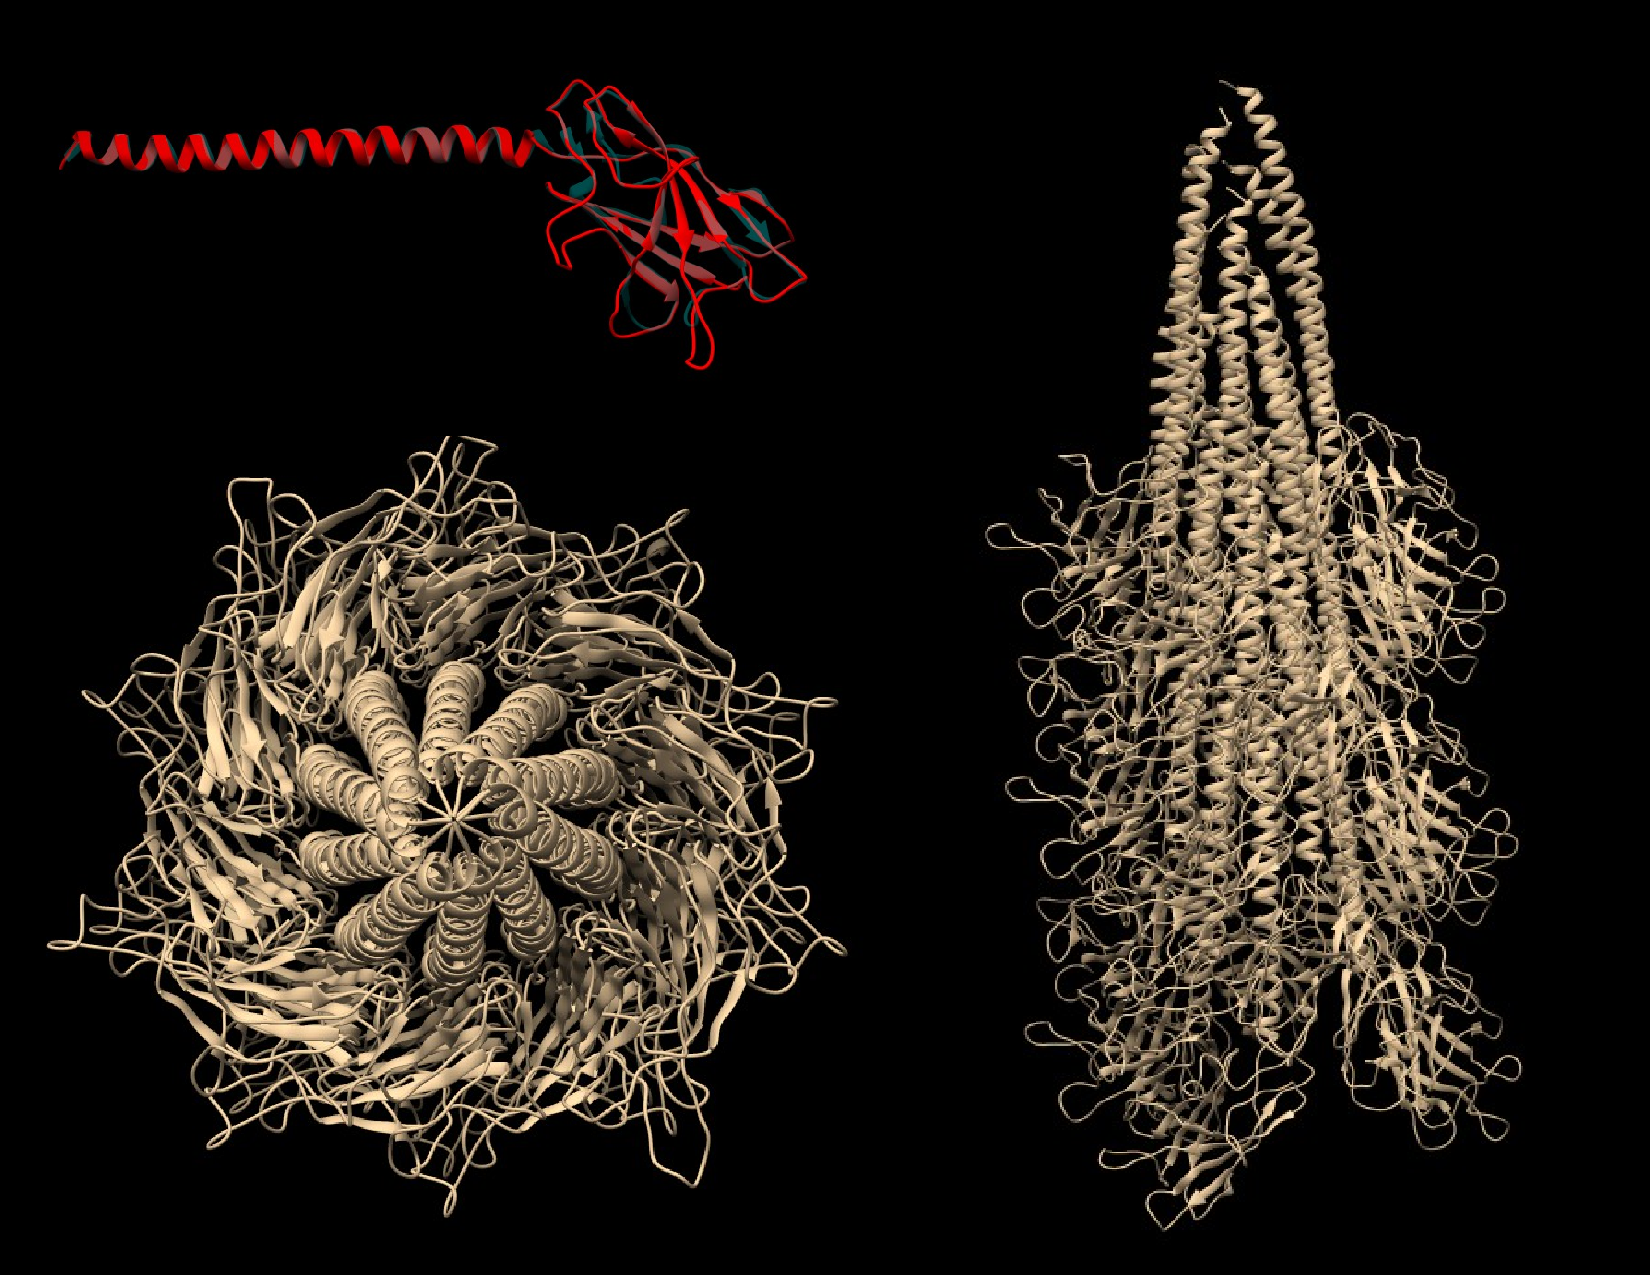
\includegraphics[width=.9\linewidth]{lacustris}  
  \caption{\textit{Methanosarcina lacustris}}
  
\end{subfigure}
\begin{subfigure}{.5\textwidth}
  \centering
  % include fourth image
  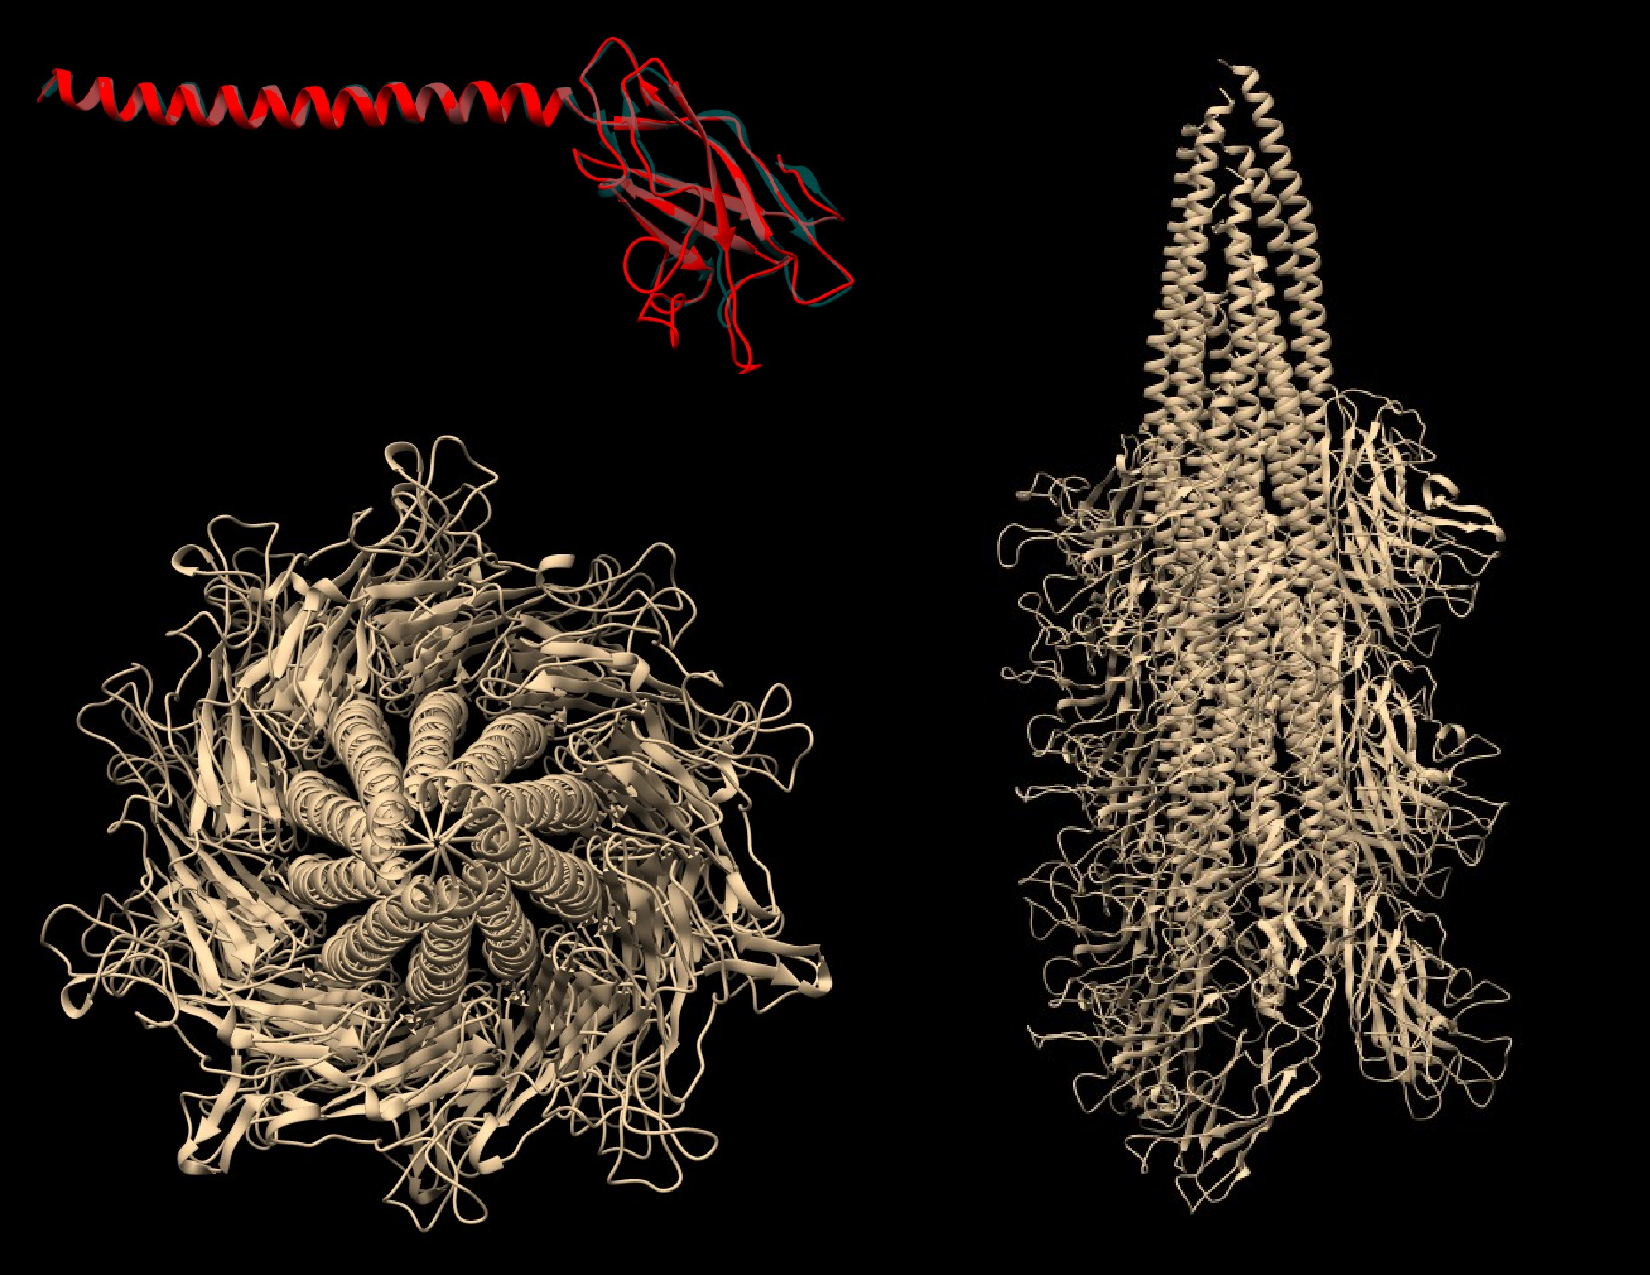
\includegraphics[width=.9\linewidth]{mazei}  
  \caption{\textit{Methanosarcina mazei}}
  
\end{subfigure}
\caption{Homology based modelling}
\label{homology}
\end{figure}













%----------------------------------------------------------------------------------------------------
%									Discussion
%----------------------------------------------------------------------------------------------------

\chapter{Discussion and Conclusion}





\section{Electromethanogenesis}

The list of methanogenic archaea obtained in this study was compared to comprehensive list of organisms involved in electromethanogenesis provided by \citet{blasco2017edge}. The result was neither inclusive of all organisms found in this study nor exclusive. If it were to be exclusive or inclusive of all the organisms found in this study, it would've strongly suggested the role of conductive archaellum as a conduit for direct electron uptake by these methanogens. Further literature search was performed to check for methanogens that were not on the list of organisms associated with electromethanogenesis but yielded no results. However  it was noted that all organisms of order Methanosarcinales found in this study were on the list of organisms associated with electromethanogenesis.

\section{DIET through E-pili}

The study by \citet{yee2020extracellular} lists all the experimentally proven syntropic DIET pairs till date and expands on it by additional six pairs. On comparison, it was found that not all methanogens that formed DIET pairs were part of results of this study suggesting presence of electrically conductive archaellum not being a necessity for DIET through E-pili. Moreover study by \citet{yee2020extracellular}  contradicts the idea of archaellum being conduit for direct electron uptake in DIET pairs by confirming and expanding on previous study by \citet{rotaru2014new} that strict hydrogenotrophs like \textit{M. hungatei} are incapable of forming DIET pairs with electrogens. All the methanogens that formed DIET pairs were of order Methanosarcinales and the study concluded that DIET is conserved only to this order. The study further hypothesized that the ability of Methanosarcinales for direct electron uptake might be property of cell surface structures.



\section{DIET through conductive material}

DIET through conductive materials have been observed in few methanogens\citep{lovley2017syntrophy} which on examination have revealed that all the methanogens are of order Methanosarcinales. Study conducted by \citet{salvador2017carbon} showed that carbon nanotubes acelerated methane production in pure cultures of methanogens including \textit{M.hungatei} but indicated no evidence of DIET.

Study conducted by \citet{holmes2021mechanisms} tested DIET pair \textit{Methanosarcina acetivorans} and \textit{Geobacter metallireducens} with and without presence archaellum in \textit{M. acetivorans}. The pair without archaellum did not form efficient DIET. Introduction of GAC showed to mitigate this problem which is known to be substitute for e-pili\citep{lovley2017syntrophy}. However the study proposed that further experiments need to be performed and traditional roles of archaella, such as conferring motility and facilitating attachment might be the reason for said observation rather than the possibility of archaellum of \textit{M. acetivorans} being conductive.


\vspace{1cm}

The above observations made indicate a strong possibility that electrical conductive archaella might not have any direct role to play in DIET in favor of hypothesis proposed by \citet{yee2020extracellular} that DIET is property of cell surface structures unique to methanogens of order Methanosarcinales. The function of electrically conductive archaella of \textit{M. hungatei} may merely be to facilitate cell attachment by dissipating charge barriers between cells and minerals/electrodes as suggested by \citet{walker2019archaellum}


\section{Other findings}

This study confirms that in euryarchaeotes archaella are characterized by the presence of multiple archaellin proteins as stated by \citet{meshcheryakov2019high} and that such multiplicity is assumed to be important for assembly of functional archaella, since deletion of individual archaellin genes often leads to non archaellated cells. They reported $\geq$5 copies being the norm but in this study it was found that \textit{M. acetivorans} which has only three copies of archaellin gene was observed to form archaella\citep{holmes2021mechanisms}. Some methanogens in results of this study have only one copy. This needs to be investigated whether they will form archaella.

The phylogenetic tree constructed based multiple squence alignment of archaellin showed that the organisms found are evolutionarily closely related which was confirmed by comparing to work by \citet{adam2017growing}.

\vspace{0.5cm}

Regarding the structure of the archaellum, this study confirms that archaellins universally possess highly structurally conserved and mostly hydrophobic N-terminal sequences which form inward facing $\alpha$ helix while C-terminal outward facing portion of the $ \beta$ barrel is hydrophilic.\citep{meshcheryakov2019high, daum2017structure, poweleit2016cryoem}. This property and the highly conserved metal binding site discovered by \citet{meshcheryakov2019high} seems to be the primary reason for archaella stability.


\vspace{2cm}
\section{Conclusion}

This study indicates a strong possibility that electrically conductive archaella might not play any direct role in DIET and supports the hypothesis that DIET  is property of cell surface structures and is unique to methanogens of order Methanosarcinales.




%----------------------------------------------------------------------------------------------------
%								Bibliography and Appendix
%----------------------------------------------------------------------------------------------------

\bibliographystyle{unsrtnat} % bibliography style. 'unsrtnat' = unsorted. check documentation of natbib package for more options

\bibliography{Bibliography} % prints bibliography. 'Bibliography' is the name of the .bib file.




%\appendix

\chapter{Appendix}\label{appendix}


\begin{table}[h]
\small
\begin{tabular}{ll}
\textit{Methanimicrococcus blatticola}   & \textit{Methanobrevibacter wolinii}      \\
\textit{Methanobacterium aarhusense}     & \textit{Methanocalculus chunghsingensis} \\
\textit{Methanobacterium alcaliphilum}   & \textit{Methanocalculus halotolerans}    \\
\textit{Methanobacterium arcticum}       & \textit{Methanocalculus pumilus}         \\
\textit{Methanobacterium beijingense}    & \textit{Methanocalculus taiwanensis}     \\
\textit{Methanobacterium bryantii}       & \textit{Methanocaldococcus fervens}      \\
\textit{Methanobacterium congolense}     & \textit{Methanocaldococcus indicus}      \\
\textit{Methanobacterium espanolae}      & \textit{Methanocaldococcus infernus}     \\
\textit{Methanobacterium ferruginis}     & \textit{Methanocaldococcus jannaschii}   \\
\textit{Methanobacterium flexile}        & \textit{Methanocaldococcus villosus}     \\
\textit{Methanobacterium formicicum}     & \textit{Methanocaldococcus vulcanius}    \\
\textit{Methanobacterium ivanovii}       & \textit{Methanocella arvoryzae}          \\
\textit{Methanobacterium kanagiense}     & \textit{Methanocella conradii}           \\
\textit{Methanobacterium lacus}          & \textit{Methanocella paludicola}         \\
\textit{Methanobacterium movens}         & \textit{Methanococcoides alaskense}      \\
\textit{Methanobacterium oryzae}         & \textit{Methanococcoides burtonii}       \\
\textit{Methanobacterium palustre}       & \textit{Methanococcoides methylutens}    \\
\textit{Methanobacterium petrolearium}   & \textit{Methanococcus aeolicus}          \\
\textit{Methanobacterium subterraneum}   & \textit{Methanococcus maripaludis}       \\
\textit{Methanobacterium thermaggregans} & \textit{Methanococcus vannielii}         \\
\textit{Methanobacterium uliginosum}     & \textit{Methanococcus voltae}            \\
\textit{Methanobacterium veterum}        & \textit{Methanocorpusculum aggregans}    \\
\textit{Methanobrevibacter acididurans}  & \textit{Methanocorpusculum bavaricum}    \\
\textit{Methanobrevibacter arboriphilus} & \textit{Methanocorpusculum labreanum}    \\
\textit{Methanobrevibacter curvatus}     & \textit{Methanocorpusculum parvum}       \\
\textit{Methanobrevibacter cuticularis}  & \textit{Methanocorpusculum sinense}      \\
\textit{Methanobrevibacter filiformis}   & \textit{Methanoculleus bourgensis}       \\
\textit{Methanobrevibacter gottschalkii} & \textit{Methanoculleus chikugoensis}     \\
\textit{Methanobrevibacter millerae}     & \textit{Methanoculleus marisnigri}       \\
\textit{Methanobrevibacter olleyae}      & \textit{Methanoculleus palmolei}         \\
\textit{Methanobrevibacter oralis}       & \textit{Methanoculleus receptaculi}      \\
\textit{Methanobrevibacter ruminantium}  & \textit{Methanoculleus submarinus}       \\
\textit{Methanobrevibacter smithii}      & \textit{Methanoculleus thermophilus}     \\
\textit{Methanobrevibacter thaueri}      & \textit{Methanofollis aquaemaris}        \\
\textit{Methanobrevibacter woesei}       & \textit{Methanofollis ethanolicus}      
\end{tabular}
\end{table}


\begin{table}[]
\small
\begin{tabular}{ll}
\textit{Methanofollis formosanus}         & \textit{Methanosarcina barkeri}                   \\
\textit{Methanofollis liminatans}         & \textit{Methanosarcina horonobensis}              \\
\textit{Methanofollis tationis}           & \textit{Methanosarcina lacustris}                 \\
\textit{Methanogenium boonei}             & \textit{Methanosarcina mazei}                     \\
\textit{Methanogenium cariaci}            & \textit{Methanosarcina semesiae}                  \\
\textit{Methanogenium frigidum}           & \textit{Methanosarcina siciliae}                  \\
\textit{Methanogenium marinum}            & \textit{Methanosarcina thermophila}               \\
\textit{Methanogenium organophilum}       & \textit{Methanosarcina vacuolata}                 \\
\textit{Methanohalobium evestigatum}      & \textit{Methanosphaera cuniculi}                  \\
\textit{Methanohalophilus euhalobius}     & \textit{Methanosphaera stadtmanae}                \\
\textit{Methanohalophilus halophilus}     & \textit{Methanosphaerula palustris}               \\
\textit{Methanohalophilus mahii}          & \textit{Methanospirillum hungatei}                \\
\textit{Methanohalophilus portucalensis}  & \textit{Methanospirillum lacunae}                 \\
\textit{Methanolacinia paynteri}          & \textit{Methanothermobacter crinale}              \\
\textit{Methanolinea mesophila}           & \textit{Methanothermobacter defluvii}             \\
\textit{Methanolinea tarda}               & \textit{Methanothermobacter marburgensis}         \\
\textit{Methanolobus bombayensis}         & \textit{Methanothermobacter tenebrarum}           \\
\textit{Methanolobus oregonensis}         & \textit{Methanothermobacter thermautotrophicus}   \\
\textit{Methanolobus profundi}            & \textit{Methanothermobacter thermoflexus}         \\
\textit{Methanolobus psychrophilus}       & \textit{Methanothermobacter thermophilus}         \\
\textit{Methanolobus taylorii}            & \textit{Methanothermobacter wolfeii}              \\
\textit{Methanolobus tindarius}           & \textit{Methanothermococcus okinawensis}          \\
\textit{Methanolobus vulcani}             & \textit{Methanothermococcus thermolithotrophicus} \\
\textit{Methanolobus zinderi}             & \textit{Methanothermus fervidus}                  \\
\textit{Methanomethylovorans hollandica}  & \textit{Methanothermus sociabilis}                \\
\textit{Methanomethylovorans thermophila} & \textit{Methanotorris formicicus}                 \\
\textit{Methanomicrobium mobile}          & \textit{Methanotorris igneus}                     \\
\textit{Methanoplanus endosymbiosus}      & \textit{Methermicoccus shengliensis}              \\
\textit{Methanoplanus limicola}           & \textit{Methanospirillum psychrodurum}            \\
\textit{Methanoplanus petrolearius}       & \textit{Methanobrevibacter boviskoreani}          \\
\textit{Methanopyrus kandleri}            & \textit{Methanobacterium movilense}               \\
\textit{Methanoregula boonei}             & \textit{Methanomethylovorans uponensis}           \\
\textit{Methanoregula formicicum}         & \textit{Methanocalculus natronophilus}            \\
\textit{Methanosaeta concilii}            & \textit{Methanohalophilus levihalophilus}         \\
\textit{Methanosaeta harundinacea}        & \textit{Methanosarcina soligelidi}                \\
\textit{Methanosaeta pelagica}            & \textit{Methanococcoides vulcani}                 \\
\textit{Methanosaeta thermophila}         & \textit{Methanospirillum stamsii}                 \\
\textit{Methanosalsum zhilinae}           & \textit{Methanomassiliicoccus luminyensis}        \\
\textit{Methanosarcina acetivorans}       & \textit{Methanoculleus horonobensis}              \\
\textit{Methanosarcina baltica}           & \textit{Methanoculleus hydrogenitrophicus}       
\end{tabular}
\end{table}





\end{document}
